\documentclass[12pt,a4paper,twoside,openright,draft]{report} %thesis

\usepackage[utf8]{inputenc}
\usepackage[english]{babel}
\usepackage{amsmath}
\usepackage{amsfonts}
\usepackage{amssymb}
\usepackage{indentfirst}
\usepackage{makeidx}
\usepackage{pdfpages}
\usepackage{amsthm}
\usepackage{stmaryrd}
\usepackage{mathtools}
\usepackage{xspace}
\usepackage{infer}
\usepackage{float}
\usepackage[all]{xy}
\usepackage{array}
\usepackage{version}
\usepackage{verbatim} 
\usepackage{balance}
\usepackage{enumerate}
\usepackage{fullpage}
\usepackage{pifont}
\usepackage[textsize=footnotesize,backgroundcolor=white,linecolor=black]{todonotes}
\usepackage[final]{listings}
\usepackage{tabularx}

\lstset{language=ml}
\lstset{commentstyle=\textit}
%\lstset{mathescape=true}
\lstset{backgroundcolor=,rulecolor=}
\lstset{tabsize=2}
%\lstset{frame=lines}
\lstset{breaklines=true}
\lstset{basicstyle=\ttfamily}
\lstset{showstringspaces=false}


\floatstyle{ruled}
\restylefloat{table}

\newtheorem{definition}{Definition}
\newtheorem{lemma}{Lemma}
\newtheorem{theorem}{Theorem}
\newtheorem{proposition}{Proposition}
\newtheorem{assumption}{Assumption}

%\DeclareExpandableDocumentCommand{\mcl2}[1]{\multicolumn{2}{l}{#1}}
%\newcommand{\mcl3}[1]{\multicolumn{3}{l}{#1}}

\author{Michele Bugliesi \and Stefano Calzavara \and Enrico Steffinlongo}
\title{Privilege separation in browser architectures}

% basics
\newcommand{\names}{\mathcal{N}}
\newcommand{\vars}{\mathcal{V}}
\newcommand{\perms}{\mathcal{P}}
\newcommand{\refs}{\mathcal{R}}
\newcommand{\caller}{\mathbf{caller}}

\renewcommand{\vec}[1]{\overrightarrow{#1}}
\newcommand{\subst}[2]{[#1/#2]}
\newcommand{\overwrite}[2]{[#1 \mapsto #2]}
\newcommand{\xra}[1]{\xrightarrow{#1}}
\newcommand{\xRa}[1]{\xRightarrow{#1}}
\newcommand{\hra}{\hookrightarrow}
\newcommand{\fv}{\mathit{fv}}
\newcommand{\fn}{\mathit{fn}}
\newcommand{\fnfv}{\mathit{fnfv}}
\newcommand{\map}[3]{#1 \stackrel{#2}{\mapsto} #3}
\newcommand{\dom}{\mathit{dom}}
\newcommand{\defined}[1]{#1\!\downarrow\ }

\newcommand{\powerset}[1]{2^{#1}}
\newcommand{\jm}{\mathcal{J}}
\newcommand{\fvbv}{\mathit{vars}}

\newenvironment{mcases}[0]{\begin{list}{{\em Case}}{\leftmargin 5pt}}{\end{list}}

% permission
\newcommand{\join}{\sqcup}
\newcommand{\meet}{\sqcap}
\newcommand{\compl}[1]{#1^*}

% values
\newcommand{\lam}[2]{\lambda #1.#2}
\newcommand{\rec}[1]{\{#1\}}
\newcommand{\unit}{\mathbf{unit}}
\newcommand{\true}{\mathbf{true}}
\newcommand{\false}{\mathbf{false}}
\newcommand{\str}[1]{``\mathit{#1}''}
\newcommand{\undef}{\mathbf{undefined}}

% expressions
\newcommand{\letexpr}[3]{\mathbf{let}\ #1 = #2\ \mathbf{in}\ #3}
\newcommand{\appl}[2]{#1\, #2}
\newcommand{\op}{\mathit{op}}
\newcommand{\cond}[3]{\mathbf{if}\ (#1)\ \{\ #2\ \}\ \mathbf{else}\ \{\ #3\ \}}
\newcommand{\while}[2]{\mathbf{while}\ (#1)\ \{\ #2\ \}}
\newcommand{\lookup}[2]{#1[#2]}
\newcommand{\store}[3]{#1[#2] = #3}
\newcommand{\delete}[2]{\mathbf{delete}\ #1[#2]}
\newcommand{\err}{\mathbf{err}}
\newcommand{\newref}[2]{\mathbf{ref}_{#1}\ #2}
\newcommand{\deref}[1]{\mathbf{deref}\ #1}
\newcommand{\setref}[2]{#1 = #2}
\newcommand{\send}[3]{\overline{#1} \langle #2 \triangleright #3 \rangle}
\newcommand{\checkperms}[2]{\mathbf{check}(#1,#2)}
\newcommand{\acquire}[1]{\mathbf{acquire}(#1)}
\newcommand{\release}[1]{\mathbf{release}(#1)}
\newcommand{\register}[3]{\mathbf{register}(#1,#2,#3)}
\newcommand{\exercise}[1]{\mathbf{exercise}(#1)}
\newcommand{\self}{\mathbf{self}}

\newcommand{\match}[2]{\mathbf{match}\ #1\ \mathbf{with}\ \{#2\}}
\newcommand{\checkp}[3]{\mathbf{check}(#1)\ \mathbf{then}\ #2\ \mathbf{else}\ #3}

% components, systems and states
\newcommand{\handler}[5]{#1(#2 \triangleleft #3:#5).#4}
\newcommand{\inst}[3]{#1\{\!|#2|\!\}_{#3}}
\newcommand{\para}[2]{#1 \parallel #2}
\newcommand{\sys}[3]{#1;#2;#3}

\newcommand{\ctx}[2]{#1\langle #2\rangle}
\newcommand{\labcall}[4]{\langle #1:#2,#3:#4 \rangle}
\newcommand{\labex}[3]{#1:#2 \gg #3}

% misc
\newcommand{\lambdaJS}{\lambda_{\mathsf{JS}}}
\newcommand{\irule}[1]{({\sc #1})}

% flow logic
\newcommand{\labs}{{\mathcal L}}
\newcommand{\absenv}{\hat{\Gamma}}
\newcommand{\absflow}{\hat{\phi}}
\newcommand{\absnet}{\hat{\Phi}}
\newcommand{\absvalues}{\hat{V}}
\newcommand{\absmem}{\hat{\mu}}
\newcommand{\abscache}{\hat{\Phi}}
\newcommand{\absassert}{\hat{L}}
\newcommand{\forms}{\Phi}
\newcommand{\terms}{\mathcal{T}}

\newcommand{\absop}{\widehat{\op}}
\newcommand{\abseq}{\widehat{eq}}
\newcommand{\absget}{\widehat{get}}
\newcommand{\absset}{\widehat{set}}
\newcommand{\absdel}{\widehat{del}}

\newcommand{\dontcare}{\diamond}
\newcommand{\abscaller}{\widehat{\caller}}
\newcommand{\msg}{\mathbb{M}}
\newcommand{\abself}{\widehat{\self}}
\newcommand{\absform}[1]{\langle #1 \rangle}
\newcommand{\hasperm}[2]{#1\ \mathsf{has}\ #2}
\newcommand{\ltrue}{\mathsf{true}}
\newcommand{\lacquire}[3]{#1 \uparrow #2,#3}
\newcommand{\lrelease}[3]{#1 \downarrow #2,#3}
\newcommand{\abstrue}{\true}
\newcommand{\absfalse}{\false}
\newcommand{\absunit}{\unit}
\newcommand{\absundef}{\undef}
\newcommand{\absrec}[1]{\langle\!| #1 |\!\rangle}
\newcommand{\abslam}[2]{\lambda #1^{#2}}
\newcommand{\absfuns}{\Lambda}

\newcommand{\absC}{{\cal C}}

% debundling
\newcommand{\avail}[1]{\mathit{Avail}_{#1}}
\newcommand{\req}[1]{\mathit{Req}_{#1}}
\newcommand{\psubst}[3]{[#1/#2]@#3}
\newcommand{\unbundle}[3]{#1 \rhd_{#2}\, #3}
\newcommand{\absE}{{\cal E}}
\newcommand{\rewrite}[1]{\succ #1}

% escalation
\newcommand{\abstack}{\hat{\Upsilon}}
\newcommand{\escalate}[1]{\,\gg #1}
\newcommand{\despite}[1]{\ \mathbf{despite}\ #1}
\newcommand{\permsleak}[1]{\mathit{Leak}_{#1}}

%other mine
\newcommand{\vat}[0]{\hat{v}}
\newcommand{\ljs}{$\lambda_{JS}$}

\makeindex

\AtBeginDocument{\renewcommand{\bibname}{References}}

\begin{document}
%\frontmatter

\maketitle
\listoftables

\begin{abstract}
In many software systems as modern web browsers the user and his sensitive data often interact with the untrusted outer world. This scenario can pose a serious threat to the user's private data and gives new relevance to an old story in computer science: providing controlled access to untrusted components, while preserving usability and ease of interaction. To address the threats of untrusted components, modern web browsers propose privilege-separated architectures, which isolate components that manage critical tasks and data from components which handle untrusted inputs. The former components are given strong permissions, possibly coinciding with the full set of permissions granted to the user, while the untrusted components are granted only limited privileges, to limit possible malicious behaviours: all the interactions between trusted and untrusted components is handled via message passing. In this thesis we introduce a formal semantics for privilege-separated architectures and we provide a general definition of privilege separation: we discuss how different privilege-separated architectures can be evaluated in our framework, identifying how different security threats can be avoided, mitigated or disregarded. Specifically, we evaluate in detail the existing Google Chrome Extension Architecture in our formal model and we discuss how its design can mitigate serious security risks, with only limited impact on the user experience. 

\end{abstract}

\tableofcontents

%\mainmatter
\chapter{Introduction}
\section{Privilege separation}
\label{sec:PriviSep}


\section{Privilege escalation attacks}
\label{sec:Escalation}

\section{Chrome extension architecture overview}
\label{sec:ExtOverview}
Web browser in the last decade experienced a massive increment of usage. Such increment, combined 

\section{Chrome extension architecture weaknesses}
\label{sec:ExtWeakness}

\section{Proposal}
\label{sec:Proposal}
\label{chap:Introduction}

\chapter{Background}
\section{Chrome extension architecture}
\label{sec:ExtDetails}
As already discussed before, a Chrome extension is a software that extends the potentiality of the browser and enhances the user experience. Such extensions are not stand-alone software, but are integrated in the browser. The integration is done through a powerful API that expose to the developer lots of functionality of the browser. Since Chrome extensions interact with web pages and with browser them are developed using the classic web-style language: JavaScript. Extension can have even HTML or CSS files and can contains various resources that can be either local or remote resources as typical in the web.

As showed in \cite{ChromeExtensionOnline} a Chrome Extension is an archive containing files of various kind like JavaScript, HTML, JSON, images and others that extends the browser features.

A basic extension is composed by a manifest file and one or more JavaScript or Html files.

\subsection{Manifest}
The manifest file \texttt{manifest.json} is a JSON-formatted file. It contains all the specification of the extension and for this reason is the entry-point of the extension. Indeed when an extension is load, the loader finds the manifest file and from it create the components of the extension. It contains two mandatory fields: \texttt{name} and \texttt{version} respectively containing the name and the version of the extension. Other important fields are:
\begin{itemize}
\item \texttt{background}: contains an object with either \texttt{script} or \texttt{page} field. The former contains the source of the content script, while the other the source of an HTML page. If the \texttt{script} field is used, the scripts are injected in a empty extension core page, while if it is used \texttt{page} the HTML document with all its elements (e.g., scripts) composes the extension core;
\item \texttt{content\_scripts}: contains a list of content script objects. Each object contains the field \texttt{matches}, a list of match patterns (Match patterns are explained below), and a field \texttt{js} containing the list of JavaScript source files to be injected;
\item \texttt{permissions}: contains a list of privileges that are requested by the extension. These can be either a host match pattern for XHR request or the name of the API needed.
\end{itemize}

Another possible field is \texttt{optional\_permissions}. It contains the list of optional permissions that the extension could require. It is used to restrict the privileges granted to the app. To use one of this permissions the background page has to explicitly require it and, after having used it, the permission has to be released. A program using the optional permissions can reduce the possible privileges escalated by an attacker.

A match pattern is a string composed of three parts: \texttt{scheme}, \texttt{host} and \texttt{path}. Each part can contain a value, or \texttt{"*"} that means all possible values. In table \ref{tab:URLPatSyn} is shown the syntax of the URL patterns; more details are reported in \cite{ChromeExtensionMatch}. In this way we can decide to inject some content scripts only on pages derived from a given match. This is used when a content script of the extension has to interact with only certain pages. For example \texttt{"*://*/*"} means all pages; \texttt{"https://*/*"} means all HTTPS pages; \texttt{"https://*.google.com/*"} means all HTTPS domains that are subdomains of google with all their possible path (e.g., \texttt{mail.google.com}, \texttt{www.google.com}, \texttt{docs.google.com/mine/index.html}).

\begin{table}[tlb]
\begin{verbatim}
<url-pattern> := <scheme>://<host><path>
<scheme> := '*' | 'http' | 'https' | 'file' | 'ftp' | 'chrome-extension'
<host> := '*' | '*.' <any char except '/' and '*'>+
<path> := '/' <any chars>
\end{verbatim}
\caption{Url pattern syntax. Table taken from \cite{ChromeExtensionMatch}}
\label{tab:URLPatSyn}
\end{table}

In table \ref{src:AManifest} we can see a manifest of a simple Chrome extension that expands the feature of moodle. We can see that the extension has an empty background page on which the file \texttt{background.js} is injected. It also has permissions \texttt{tabs} and \texttt{download}, and can execute XHR to pages with every path in \texttt{https://moodle.dsi.unive.it/}. It has also one content script that is injected in all subpages of \texttt{https://moodle.dsi.unive.it/}.
\begin{table}[tlb]
\lstset{language=java,showstringspaces=false}
\begin{small}
\begin{lstlisting}
{
	"manifest_version": 2,
	"name":"Moodle expander",
	"description":"Download homework and uploads marks from a JSON string",
	"version":"1",
	"background": { "scripts": ["background.js"] },
	"permissions":  
		[
			"tabs",
			"downloads",
			"https://moodle.dsi.unive.it/*"
		],
	"content_scripts": 
		[
			{
				"matches": ["https://moodle.dsi.unive.it/*"],
				"js": ["myscript.js"]
			}
		]
}
\end{lstlisting}
\end{small}
\caption{A manifest file}
\label{src:AManifest}
\end{table}

\subsection{Content scripts}
Content scripts are JavaScript source files that are automatically injected to the web page if this matches with the pattern defined in the manifest. Otherwise it can be programmatically injected by a background page using the \texttt{chrome.tabs.executeScript} call (the function requires \texttt{tabs} permission). In the example of table \ref{tab:URLPatSyn} the JavaScript file \texttt{myscript.js} is injected to all sub-pages of \texttt{https://moodle.dsi.unive.it/}. In the extension framework content scripts are designed to interact with pages. Since this interaction could be the entry point for an attacker, content scripts have no permissions except the one used to communicate with the extension core. In order to reduce injection of code in the content script from a malign page, there is a strong isolation between the heaps of these two. Content scripts of the same extension are run together in their own address space, and the only way they have to interact with the page on which they are injected is via the DOM API. DOM API lets the content scripts access and modify only standard fields of the DOM object, while other changes are kept locally\cite{ChromeExtSpec}. This strong isolation mitigate the risk of code injection since it blocks almost completely pointer exchange. In figure \ref{fig:SepWorlds} is showed such relation.

\begin{figure}[htb]
    \centering
    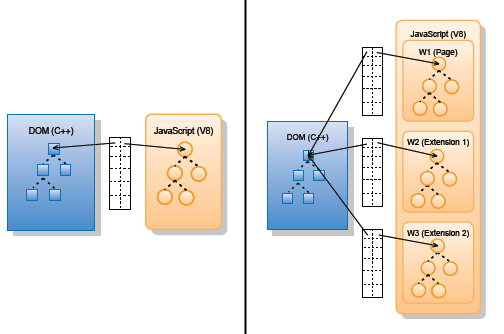
\includegraphics[scale=1]{Both}
    \caption{On the left the normal one-to-one relation between DOM implementation and JavaScript representation; On the right the one-to-many relation caused by running content scripts in isolated worlds. Figure taken from \cite{ChromeExtSpec}}
    \label{fig:SepWorlds}
\end{figure}

In order to keep functionality of extensions, communication between content scripts and extension core is done using a message passing interface. The message passing interface has crucial importance in this work since it is the only way for a content script to trigger execution of a privilege. We will discuss it later in \ref{subs:MPI}.

\subsection{Extension core}
The extension core is the most critical part of the application. It is executed in a unique origin like \texttt{chrome-extension://hcdmlbjlcojpbbinplfgbjodclfijhce} in order to prevent cross origin attacks, but it can communicate with all origins that match with one of the host permission defined in the manifest. In this environment are executed all scripts defined in the background field of the manifest. Since background pages can have remote resources of every kind (even scripts), they can also request to the web such resources, but this can be very dangerous. In fact if the resources are on HTTP connections these can be altered by an attacker. \cite{ChromeExtSpecSnd} describes how to enforce the security policy in order to avoid such possible weakness. Background pages can interact with content scripts via message passing.
%\missingfigure{Maybe figura schema Chrome Extensions comm \& elements.}

\subsection{Message passing API}
\label{subs:MPI}
Every content script of the extension can use the message passing interface. To do this it has to use the functions contained in the \texttt{chrome.runtime} object \cite{ChromeExtensionRuntime} that exposes such API.

The main way to send a message to the extension core is invoking the method \texttt{chrome.runtime.sendMessage}. Like all Chrome APIs even the message passing is asynchronous. As primary arguments it takes the message that can be of any kind and a callback function that is triggered if someone answer to the message. Before sending, the message is marshaled using a JSON serializer.

In order to listen to incoming messages, a component has to register a function on the \texttt{chrome.runtime.onMessage} event. This function will be triggered when a message arrives. Its arguments are the message (unmarshalled by the API), the sender and an optional callback used to send response to the sender of the message. The sender field is very important because it is the only way to know the real identity of the sender. In fact the message may not be used to decide the sender, because it can be of every kind.

Since content scripts are multiple and injected in various pages (tabs), the extension core for sending a message has to use the \texttt{sendMessage} method of the \texttt{tab} object to which the message has to be sent. Its behavior is the same of the \texttt{chrome.runtime.sendMessage} method.

In table \ref{tab:MPIMessage} we can see how to use the simple message passing interface. A component simply sends the message and wait for a response. The other registers \texttt{onMessage} function in the event listener \texttt{onMessage}. When the handler is triggered by an incoming message \texttt{onMessage} function it checks the message and decides to compute something according to the request or refuses the message doing nothing.

Another way to communicate, that is more secure, is using channels as in table \ref{tab:MPIPort}. In the message passing API there is a method called \texttt{connect} that triggers the corresponding event listener \texttt{onConnect} and returns a port. It has as optional arguments the name of the channel that is creating. A port object is a bidirectional channel that can be used to communicate. It contains the methods \texttt{postMessage}, \texttt{disconnect} and the events \texttt{onMessage} and \texttt{onDisconnect}. Communication using ports instead of the classical \texttt{chrome.runtime.sendMessage} is more secure, because only who has one of the port endpoint can communicate. Obviously ports are not serializable, so it is impossible to leak the ownership of a port. Ports provide a guarantee for the sender of the message.

\lstset{language=java,showstringspaces=false}
\begin{table}[htb]
\begin{small}
\begin{center}
\begin{tabular}{p{0.45\linewidth} | p{0.45\linewidth}}
Sender & Receiver\\
\hline
\begin{lstlisting} 
var info = "hello";
var callback = 
	function(response) 
	{ 
		console.log("get response: " + response);
	};
chrome.runtime.sendMessage(info, callback);
\end{lstlisting}&
\begin{lstlisting} 
var onMessage = 
	function(message, sender, sendResponse) 
	{ 
		if (message = "hello") 
		{
		    //compute message
			sendResponse("hi");
		}
		else 
			console.log("connection refused from"+sender);
	};
chrome.runtime.onMessage.addListener(onMessage);
\end{lstlisting}\\
\end{tabular}
\end{center}
\end{small}
\caption{Sending a message.}
\label{tab:MPIMessage}
\end{table}

\begin{table}[htb]
\begin{small}
\begin{center}
\begin{tabular}{p{0.45\linewidth} | p{0.45\linewidth}}
Port opening active & Port opening passive\\
\hline
\begin{lstlisting} 
var port = chrome.runtime.connect({name: "cs1"});
port.onMessage.addListener(onMessage)
port.postMessage("hi")
\end{lstlisting}&
\begin{lstlisting} 
var scriptPort = null;
var onConnect = 
	function(port) 
	{ 
		if (port.name = "cs1") 
		{
			scriptPort = port;
			port.onMessage.addListener(onMessage);
		} 
		else 
		{
			console.log("connection refused"); 
			port.disconnect();
		}
	};
chrome.runtime.onConnect.addListener(onConnect)
\end{lstlisting}\\
\end{tabular}
\end{center}
\end{small}
\caption{Port creation.}
\label{tab:MPIPort}
\end{table}

\section{Permission bundling}
\label{sec:BundlingExample}
Modern privilege-separated architectures mitigates various attacks coming from the external untrusted world, but they still have weakness. A great part of this weakness derive from bad-practice of developers that often are not security experts. One of this is called bundling. Bundling is, as the name suggests, the practice of clustering in the same component different privileges. This can be very dangerous because an attacker that compromise the bundled component can escalate all privileges clustered in it. 

In Chrome extensions sometimes programmers tend to aggregate in a single function various privileges that are delegated to different components. Moreover, often, the bundled function is the \texttt{onMessage} listener in the background, that is the entry point for an attacker that has compromised a content script. The \texttt{onMessage} function is, indeed, critical because it receives  messages from a possible compromised content script, since attacker cannot access directly the background page from the web thanks to the privilege separated and strong isolation behavior of the architecture. The practice of permission bundling, especially in the \texttt{onMessage} function is very dangerous because an attacker that compromises a content script can directly trigger the listener in order to escalate privileges. 

To reduce the attack surface exposed by bundled components, is important to base the decision of which privilege has to be exercised on trusted elements. Indeed, as seen in table \ref{tab:MPIMessage}, the choice taken by the bundled component when a message is received can depend on various factors decided by the programmer.

Let us explain the example in \ref{tab:Bundled}: suppose to have three components Background, CS1 and CS2. CS1 can only send messages that has \texttt{"getPasswd"} as title and CS2 only \texttt{"executeXHR"}. Here the Background deduct the sender checking the title of the messages instead of of explicitly checking the argument \texttt{sender}. According to the check decides which privilege has to be executed. This practice exposes all the weakness of the bundling and is very dangerous because an attacker can compromise just one of the two content scripts and from that one can forge messages with any form to escalate a permission that it does not have in the original setting.

To mitigate such weakness, in chrome extensions, is important to check the sender field of the \texttt{onMessage} function in order to be sure of the sender. This cannot be enough because, as discussed before, contents script that are injected on the same page share their memory, tab and origin, and the message passing interface are does not distinguish them. The fix of this weakness is to use ports instead of the \texttt{chrome.runtime.sendMessage} function in order to have different listener for each content script. In this way we unbundle the \texttt{onMessage} function, separating in the various listeners privileges. In table \ref{tab:UnBundled} are showed a not dangerous bundled code, and an unbundled code.

\begin{table}[htb]
\begin{small}
\begin{center}
\begin{tabular}{p{0.95\linewidth}}
Background\\
\hline
\begin{lstlisting}
function onMessage(message, sender, response)
{    	
	switch (message.title) {
		/* Requests from content script 1 */
		case "getPasswd":
		// get passwords
		response(passwd)
		break;
		
		/* Requests from content script 2 */
		case "executeXHR":
		var host = message.host
		var m = message.content;
		// execute XHR on args
		break;
				
		default:
		throw "Invalid request from contentScript";
	}
}
\end{lstlisting}\\
\hline
\hline
Content script CS1 \\
\hline
\begin{lstlisting}
var mess = {title: "getPasswd"};
chrome.runtime.sendMessage(mess);
\end{lstlisting}\\
\hline
\hline
Content script CS2\\
\hline
\begin{lstlisting}
var mess = {title: "executeXHR", host: "www.google.com", content: "hi there"};
chrome.runtime.sendMessage(mess);
\end{lstlisting}\\
\end{tabular}
\end{center}
\end{small}
\caption{Bundled code.}
\label{tab:Bundled}
\end{table}
\begin{table}[htb]
\begin{small}
\begin{center}
\begin{tabular}{p{0.95\linewidth}}
Unbundling checking sender\\
\hline
\begin{lstlisting}
function onMessage(message, sender, response)
{    	
	switch (sender) {
		/* Requests from content script 1 */
		case CS1:
		// get passwords
		response(passwd)
		break;
		
		/* Requests from content script 2 */
		case CS2:
		var host = message.host
		var m = message.content;
		// execute XHR on args
		break;
				
		default:
		throw "Invalid request from contentScript";
	}
}
\end{lstlisting}\\
\hline
\hline
Unbundling using ports.\\
\hline
\begin{lstlisting}
// Handler for messages from CS1
function onMessage_cs1(message, sender, response)
{    	
	/* Requests is content script 1 since it is on its port */
	// get passwords
	response(passwd)
}
// Handler for messages from CS2
function onMessage_cs2(message, sender, response)
{    	
	/* Requests is content script 2 since it is on its port */
	var host = message.host
	var m = message.content;
	// execute XHR on args
}
port_cs1.onMessage.addListener(onMessage_cs1);
port_cs2.onMessage.addListener(onMessage_cs2);
\end{lstlisting}\\
\hline
\end{tabular}
\end{center}
\end{small}
\caption{Unbundling.}
\label{tab:UnBundled}
\end{table}

%The existence of the undefined value and im-
%plicit type coercions in the language means that even minor
%spelling errors, for example in a property name, often has
%surprising consequences at runtime. With statically typed
%languages, the type systems provide a strong foundation for
%detecting such errors. In contrast, because of the dynamic
%nature of JavaScript web application code, our analysis must
%be capable of reasoning about the flow of control and data
%throughout the applications.

\section{Flow logic}
\label{sec:FlowLogic}
The goal of this work is to develop an analysis that is able to detect statically absence of bundling in real Chrome extensions. Moreover we want to do this automatically, so without any effort for the developer (e.g., code annotations or similar). Statically typed languages are easier to check because the typing discipline provide strong foundation for detecting the behavior of a program. On the contrary, the weak dynamically typed nature of JavaScript code makes the analysis more difficult. Since extension are written in JavaScript we have to face with problem deriving from a dynamic and weak typing discipline. Indeed, in JavaScript there are lots of quirks that made the analysis very hard with a classical typing approach. For example local and global scoping, passage of functions, and access of a property of an object using a string are very hard to handle statically. To achieve our purpose the analysis must track the flow of both control and data during the execution. In this scenario we used the flow logic approach because of its flexibility, high potential and easiness to use.

Flow logic, introduced in \cite{FlowLogic}, is a static analysis approach that derives from state of the art in program verification and has been successfully used in research projects \cite{CarmelFlowLogic,CarmelFlowLogicFormalization}. It has its root in classical approaches of static program analysis \cite{PrincipleProgramAnalysis} like control flow analysis \cite{CMLCFA}, abstract interpretation, constraint based analysis and data flow analysis. Flow logic lets the specification to focus on when an analysis estimate is acceptable, instead of how to compute such estimate. Another property is that, like structural operational semantics, is adaptable to lots of programming paradigms. Finally it can be used with various levels of abstraction according to the implementation details that are needed, but can be easily translated from one level to another. 

The principal levels of abstraction are grouped in some possible approaches: abstract versus compositional and succinct versus verbose. The abstract style is closer to standard semantics while the compositional one is more syntax directed. The succinct approach is similar to the typical style of type systems because it focuses the top part of the analysis, while the verbose approach traces all the internal information in cashes and are typical of the implementation of control flow analysis and constraint based analysis.

The modularity fits very well for analysis, because the abstract succinct style is very clean and expressive without dealing with implementation details, and from such specification is easy to commute it to a compositional verbose specification. From the latter is possible to build an algorithm for generating the set of constraints of a program and combining it with a simple constraint solver like the worklist algorithm \cite{PrincipleProgramAnalysis} or with a more sophisticated ones like the succinct solver \cite{SuccinctSolver} or the BANSHEE solver \cite{BansheeSolver}, is possible to compute the estimate for a program.

Let us have an example: suppose to have a program and ``magically'' an estimate for it: using flow logic judgments we are able to establish if such estimate respect our analysis for the program, or not. This decision is granted by the fact that one of the constraint of generated by the constraint generator is not satisfied. Moreover we can compute starting from the constraint an estimate that satisfy the analysis.

In this work, is used the flow logic, and as described before, the various specification-to-implementation steps are done. In chapter \ref{chap:Formalization} is used an abstract-succinct approach, and in chapter \ref{chap:Implementation} the analysis is expanded in the compositional-verbose one; from this the algorithm for constraint-generation is built and finally is used a worklist algorithm to solve the constraints and to find an estimate for a program.

\section{Lambda JS}
Since JavaScript is a real world programming language that has high level constructs, weak and dynamic typing discipline and unconventional semantics, it is very complex to analyze. We reduce JavaScript to \ljs\ as described in \cite{LambdaJS}. \ljs\ is a dialect of Scheme, with a small-step operational semantics, that, in contrast with JavaScript, has few standard constructs taken from the lambda calculus. \ljs\ models features of JavaScript in a way that corresponds closely to well known languages semantics.

Thanks to this we can simplify a lot the analysis without losing expressiveness because \ljs\ contains just few construct with simple semantics.

Unfortunately \ljs\ is not proved to be a sound representation of JavaScript, but all test on desugared file showed that its semantic coincide with JavaScript. In figure \ref{asm:LJS} is shown the testing method adopted to validate semantics of \ljs.

\begin{figure}[htb]
    \centering
    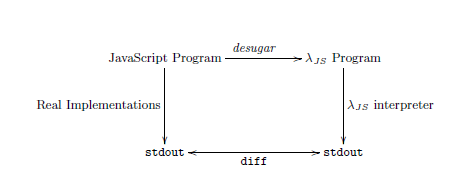
\includegraphics[scale=1]{LambdaJS}
    \caption{The \ljs\ test. Figure taken from \cite{LambdaJS}}
    \label{fig:LJS}
\end{figure}
\label{chap:Background}

\chapter{Formalization}
\section{Calculus}
\label{sec:Calculus}

\section{Safety properties} %proprietà di sicurezza
\label{sec:SafetyProp}

\section{Analysis specification} %specifica dell'analisi
\label{sec:AnalysisSpec}
\subsection{Abstract succinct}
\[
\begin{array}{llcl}
\mathit{Abstract\ cache} & \Cat & : & \labs \rightarrow \absvalues \\
\mathit{Abstract\ variable\ environment} & \Env & : & \vars \rightarrow \absvalues \\
\mathit{Abstract\ memory} & \absmem & : & \labs \times \perms \rightarrow \absvalues \\
\mathit{Abstract\ permission\ cache} & \Pat & : & \labs \rightarrow \perms \\
\end{array}
\]
\begin{tabular}{l l l l}
{[\textit{PE-Val}]}&\multicolumn{3}{l}{$\aenvs \modelrho c : \vat$ iff $\{d_c\} \subseteq \vat$} \\
{[\textit{PE-Var}]}&\multicolumn{3}{l}{$\aenvs \modelrho x : \vat$ iff $\Env(x) \subseteq \vat$} \\ 
{[\textit{PE-Lambda}]}&\multicolumn{3}{l}{$\aenvs \modelrho \lam{x}{e} : \vat$ iff $\{\lam{x}{e}\} \subseteq \vat$} \\
{[\textit{PE-Obj}]}&\multicolumn{3}{l}{$\caest {\rec{\vec{str_i : e_i}}}$ iff} \\
&&\multicolumn{2}{l}{$\forall i: \caesti {e_i} {i} \wedge$}\\
&&&$\rec{\vec{str_i :\vat_i}} \subseteq \vat \wedge$ \\
&&&$\rho_i \sqsubseteq \rho$ \\ 
{[\textit{PE-Let}]}&\multicolumn{3}{l}{$\caest {\letexprs{x_i}{e_i}{e'}}$ iff}\\
&&\multicolumn{2}{l}{$\aenvs \modelrho e' : \vat \gg \rho' \wedge$} \\
&&\multicolumn{2}{l}{$\rho' \sqsubseteq \rho \wedge$} \\
&&\multicolumn{2}{l}{$ \forall i:$}\\
&&& $\caesti {e_i} {i} \wedge$ \\
&&& $\vat_i \subseteq \Env(x_i) \wedge$ \\
&&& $\rho_i \sqsubseteq \rho$ \\
{[\textit{PE-App}]}&\multicolumn{3}{l}{$\caest {\appl {e_1} {e_2}}$ iff} \\
&&\multicolumn{2}{l}{$\caesti {e_1} {1} \wedge$} \\
&&\multicolumn{2}{l}{$\caesti {e_2} {2} \wedge$} \\
&&\multicolumn{2}{l}{$\rho_1 \sqsubseteq \rho \wedge$} \\
&&\multicolumn{2}{l}{$\rho_2 \sqsubseteq \rho \wedge$} \\
&&\multicolumn{2}{l}{$\forall (\lam{x}{e_0}) \in \vat_1 :$}\\
&&&$\vat_2 \subseteq \Env(x) \wedge$\\
&&&$\caesti {e_0} {0} \wedge$\\ 
&&&$\rho_0 \sqsubseteq \rho \wedge$\\
&&&$\vat_0 \subseteq \vat $\\
{[\textit{PE-Op}]}&\multicolumn{3}{l}{$\caest {\op (\vec{e_i})} $ iff}\\
&&\multicolumn{2}{l}{$\forall i :$}\\
&&&$\caesti {e_i} {i} \wedge $\\
&&&$\rho_i \sqsubseteq \rho \wedge$\\
&&\multicolumn{2}{l}{$\widehat{op} (\vec{\vat_i}) \subseteq \vat $}\\
{[\textit{PE-Cond}]}&\multicolumn{3}{l}{$\caest {\cond {e_0} {e_1} {e_2}} $ iff}\\
&&\multicolumn{2}{l}{$\caesti {e_0} {0} \wedge$}\\
&&\multicolumn{2}{l}{$\rho_0 \sqsubseteq \rho \wedge$} \\
&&\multicolumn{2}{l}{$\widehat{\true} \in \vat_0 \Rightarrow$}\\
&&&$\caesti {e_1} {1} \wedge \vat_1 \subseteq \vat \wedge \rho_1 \sqsubseteq \rho \wedge$ \\
&&\multicolumn{2}{l}{$\widehat{\false} \in \vat_0 \Rightarrow$}\\
&&&$\caesti {e_2} {2} \wedge \vat_2 \subseteq \vat \wedge \rho_2 \sqsubseteq \rho$ \\
{[\textit{PE-While}]}&\multicolumn{3}{l}{$\caest {\while {e_1} {e_2}} $ iff}\\
&&\multicolumn{2}{l}{$\caesti {e_1} {1} \wedge $}\\
&&\multicolumn{2}{l}{$\rho_1 \sqsubseteq \rho \wedge$} \\
&&\multicolumn{2}{l}{$\widehat{\true} \in \vat_1 \Rightarrow$}\\
&&&$\caesti {e_2} {2} \wedge \vat_2 \subseteq \vat \wedge \rho_2 \sqsubseteq \rho \wedge$\\
&&\multicolumn{2}{l}{$\widehat{\false} \in \vat_1 \Rightarrow$}\\
&&&$\widehat{\undef} \subseteq \vat$\\
{[\textit{PE-GetField}]}&\multicolumn{3}{l}{$\caest {\lookup {e_1} {e_2}} $ iff}\\
&&\multicolumn{2}{l}{$ \caesti {e_1} {1} \wedge $}\\
&&\multicolumn{2}{l}{$\rho_1 \sqsubseteq \rho \wedge$} \\
&&\multicolumn{2}{l}{$ \caesti {e_2} {2} \wedge $} \\
&&\multicolumn{2}{l}{$\rho_2 \sqsubseteq \rho \wedge$} \\
&&\multicolumn{2}{l}{$\widehat{get} (\vat_1, \vat_2) \subseteq \vat$} \\
\end{tabular}\newpage
\begin{tabular} {l l l l}
{[\textit{PE-SetField}]}&\multicolumn{3}{l}{$\caest {\store {e_0} {e_1} {e2}} $ iff}\\
&&\multicolumn{2}{l}{$ \caesti {e_0} {0} \wedge $}\\
&&\multicolumn{2}{l}{$\rho_0 \sqsubseteq \rho \wedge$} \\
&&\multicolumn{2}{l}{$ \caesti {e_1} {1} \wedge $} \\
&&\multicolumn{2}{l}{$\rho_1 \sqsubseteq \rho \wedge$} \\
&&\multicolumn{2}{l}{$ \caesti {e_2} {2} \wedge $} \\
&&\multicolumn{2}{l}{$\rho_2 \sqsubseteq \rho \wedge$} \\
&&\multicolumn{2}{l}{$\widehat{set} (\vat_0, \vat_1, \vat_2) \subseteq \vat$} \\
{[\textit{PE-DelField}]}&\multicolumn{3}{l}{$\caest {\delete {e_1} {e_2}} $ iff}\\
&&\multicolumn{2}{l}{$ \caesti {e_1} {1} \wedge$}\\
&&\multicolumn{2}{l}{$\rho_1 \sqsubseteq \rho \wedge$} \\
&&\multicolumn{2}{l}{$ \caesti {e_2} {2} \wedge $} \\
&&\multicolumn{2}{l}{$\rho_2 \sqsubseteq \rho \wedge$} \\
&&\multicolumn{2}{l}{$\widehat{del} (\vat_1, \vat_2) \subseteq \vat$}\\
{[\textit{PE-Ref}]}&\multicolumn{3}{l}{$ \aenvs \modelrho \newref {r,\rho_r} {e} :\{r\} \gg \rho $ iff}\\
&&\multicolumn{2}{l}{$ \caest {e} \wedge $}\\
&&\multicolumn{2}{l}{$\rho_r \sqsubseteq \rho_s \Rightarrow \vat \subseteq \muat(r, \rho_r) $} \\
{[\textit{PE-DeRef}]}&\multicolumn{3}{l}{$\caest {\deref {e}} $ iff}\\
&&\multicolumn{2}{l}{$\caesti {e} {1} \wedge $}\\
&&\multicolumn{2}{l}{$\rho_1 \sqsubseteq \rho \wedge$ }\\
&&\multicolumn{2}{l}{$\forall r \in \vat_1 : \forall \rho_r \sqsubseteq \rho_s : \muat(r, \rho_r) \subseteq \vat$ }\\
{[\textit{PE-SetRef}]}&\multicolumn{3}{l}{$\caest {\setref {e_1} {e_2}} $ iff}\\
&&\multicolumn{2}{l}{$ \caesti {e} {1} \wedge $}\\
&&\multicolumn{2}{l}{$\rho_1 \sqsubseteq \rho \wedge$} \\
&&\multicolumn{2}{l}{$ \caesti {e_2} {2} \wedge $}\\
&&\multicolumn{2}{l}{$\rho_2 \sqsubseteq \rho \wedge$}\\
&&\multicolumn{2}{l}{$\forall r \in \vat_1 : \forall \rho_r \sqsubseteq \rho_s :$}\\
&&&$\vat_2 \subseteq \muat(r, \rho_r) \wedge$ \\
&&&$\vat_2 \subseteq \vat $\\
{[\textit{PE-Send}]}& \dots \\
{[\textit{PE-Err}]}& \dots \\
{[\textit{PE-Exercise}]}& \dots \\
\end{tabular}

\subsection{Compositional Verbose}
\begin{tabular}{l l l l}
{[\textit{CV-Val}]}&\multicolumn{3}{l}{$ \ccestl {c} $ iff $\{d_c\} \subseteq \Cat(\ell)$} \\ 
{[\textit{CV-Var}]}&\multicolumn{3}{l}{$ \ccestl {x} $ iff $\Env(x) \subseteq \Cat(\ell)$} \\ 
{[\textit{CV-Lambda}]}&\multicolumn{3}{l}{$ \ccestl {\lam{x}{\lbt 0}} $ iff}\\
&&\multicolumn{2}{l}{$\{\lam{x}{\lbt 0}\} \subseteq \Cat(\ell) \wedge $}\\
&&\multicolumn{2}{l}{$ \ccest {\lbt 0}$}\\
{[\textit{CV-Obj}]}&\multicolumn{3}{l}{$ \ccestl {\rec{\vec{str_i : \lbt i}}}$ iff}\\
&&\multicolumn{2}{l}{$\forall i:$}\\
&&&$\ccest {\lbt i} \wedge$\\
&&&$\Pat(\ell_i) \sqsubseteq \Pat(\ell) \wedge$\\ 
&&\multicolumn{2}{l}{$\rec{\vec{str_i : \Cat(\ell_i)}} \subseteq \Cat_\ell $} \\
{[\textit{CV-Let}]}&\multicolumn{3}{l}{$ \ccestl {\letexprs{x_i}{\lbt i}{{e'}^{\ell'}}}$ iff}\\
&&\multicolumn{2}{l}{$ \ccest {{e'}^{\ell'}} \wedge$} \\
&&\multicolumn{2}{l}{$ \Pat(\ell') \sqsubseteq \Pat(\ell) \wedge$}\\
&&\multicolumn{2}{l}{$ \Cat(\ell') \subseteq \Cat(\ell) \wedge$}\\
&&\multicolumn{2}{l}{$ \forall i:$}\\
&&&$\ccest {{e_i}^{\ell_i}} \wedge$ \\
&&& $ \Cat(\ell_i) \subseteq \Env(x_i) \wedge$ \\
&&& $ \Pat(\ell_i) \sqsubseteq \Pat(\ell) $ \\
{[\textit{CV-App}]}&\multicolumn{3}{l}{$ \ccestl {\appl {\lbt 1} {\lbt 2}}$ iff}\\
&&\multicolumn{2}{l}{$\ccest {\lbt 1} \wedge \ccest {\lbt 2} \wedge$} \\
&&\multicolumn{2}{l}{$\Pat(\ell_1) \sqsubseteq \Pat(\ell) \wedge \Pat(\ell_2) \sqsubseteq \Pat(\ell)$} \\
&&\multicolumn{2}{l}{$\forall (\lam{x}{\lbt 0}) \in \Cat(\ell_1) :$}\\
&&&$\Cat(\ell_2) \subseteq \Env(x) \wedge \Cat(\ell_0) \subseteq \Cat(\ell) \wedge$\\
&&&$\Pat(\ell_0) \sqsubseteq \Pat(\ell) $\\
{[\textit{CV-Op}]}&\multicolumn{3}{l}{$ \ccestl {\op (\vec{\lbt i})} $ iff}\\
&&\multicolumn{2}{l}{$\forall i :$}\\
&&&$\ccest {\lbt i} \wedge $\\
&&&$\Pat(\ell_i) \sqsubseteq \Pat(\ell) \wedge$\\
&&\multicolumn{2}{l}{$\widehat{op} (\Cat(\ell_i)) \subseteq \Cat(\ell) $}\\
{[\textit{CV-Cond}]}&\multicolumn{3}{l}{$\ccestl{\cond {\lbt 0} {\lbt 1} {\lbt 2}} $ iff}\\
&&\multicolumn{2}{l}{$ \ccest {\lbt 0} \wedge $}\\
&&\multicolumn{2}{l}{$\Pat(\ell_0) \sqsubseteq \Pat(\ell) \wedge$} \\
&&\multicolumn{2}{l}{$\widehat{\true} \in \Cat(\ell_0) \Rightarrow$}\\
&&&$\ccest {\lbt 1} \wedge \Cat(\ell_1) \subseteq \Cat(\ell)\wedge$\\
&&&$\Pat(\ell_1) \sqsubseteq \Pat(\ell) \wedge$ \\
&&\multicolumn{2}{l}{$\widehat{\false} \in \Cat(\ell_0) \Rightarrow$}\\
&&&$\ccest {\lbt 2} \wedge \Cat(\ell_2) \subseteq \Cat(\ell) \wedge$\\
&&&$\Pat(\ell_2) \sqsubseteq \Pat(\ell)$ \\
{[\textit{CV-While}]}&\multicolumn{3}{l}{$\ccestl {\while {\lbt 1} {\lbt 2}} $ iff}\\
&&\multicolumn{2}{l}{$ \ccest {\lbt 1} \wedge $}\\
&&\multicolumn{2}{l}{$\Pat(\ell_1) \sqsubseteq \Pat(\ell) \wedge$} \\
&&\multicolumn{2}{l}{$\widehat{\true} \in \Cat(\ell_1) \Rightarrow$}\\
&&&$\ccest {\lbt 2} \wedge \Cat(\ell_2) \subseteq \Cat(\ell) \wedge$\\
&&&$ \Pat(\ell_2) \sqsubseteq \Pat(\ell) \wedge$\\
&&\multicolumn{2}{l}{$\widehat{\false} \in \Cat(\ell_1) \Rightarrow \widehat{\undef} \subseteq \Cat(\ell)$}\\
\end{tabular}

\begin{tabular} {l l l l}
{[\textit{CV-GetField}]}&\multicolumn{3}{l}{$\ccestl {\lookup {\lbt 1} {\lbt 2}} $ iff}\\
&&\multicolumn{2}{l}{$ \ccest {\lbt1} \wedge $}\\
&&\multicolumn{2}{l}{$\Pat(\ell_1) \sqsubseteq \Pat(\ell) \wedge$} \\
&&\multicolumn{2}{l}{$ \ccest {\lbt 2} \wedge $} \\
&&\multicolumn{2}{l}{$\Pat(\ell_2) \sqsubseteq \Pat(\ell) \wedge$} \\
&&\multicolumn{2}{l}{$\widehat{get} (\Cat(\ell_1), \Cat(\ell_2)) \subseteq \Cat(\ell)$} \\
{[\textit{CV-SetField}]}&\multicolumn{3}{l}{$\ccestl {\store {\lbt 0} {\lbt 1} {\lbt 2}} $ iff}\\
&&\multicolumn{2}{l}{$ \ccest {\lbt 0} \wedge $}\\
&&\multicolumn{2}{l}{$\Pat(\ell_0) \sqsubseteq \Pat(\ell) \wedge$} \\
&&\multicolumn{2}{l}{$ \ccest {\lbt 1} \wedge $} \\
&&\multicolumn{2}{l}{$\Pat(\ell_1) \sqsubseteq \Pat(\ell) \wedge$} \\
&&\multicolumn{2}{l}{$ \ccest {\lbt 2} \wedge $} \\
&&\multicolumn{2}{l}{$\Pat(\ell_2) \sqsubseteq \Pat(\ell) \wedge$} \\
&&\multicolumn{2}{l}{$\widehat{set} (\Cat(\ell_0), \Cat(\ell_1), \Cat(\ell_2)) \subseteq \Cat(\ell)$} \\
{[\textit{CV-DelField}]}&\multicolumn{3}{l}{$\ccestl {\delete {\lbt 1} {\lbt 2}} $ iff}\\ 
&&\multicolumn{2}{l}{$ \ccest {\lbt 1} \wedge $}\\
&&\multicolumn{2}{l}{$\Pat(\ell_1) \sqsubseteq \Pat(\ell) \wedge$} \\
&&\multicolumn{2}{l}{$ \ccest {\lbt 2} \wedge $} \\
&&\multicolumn{2}{l}{$\Pat(\ell_2) \sqsubseteq \Pat(\ell) \wedge$} \\
&&\multicolumn{2}{l}{$\widehat{del} (\Cat(\ell_1), \Cat(\ell_2)) \subseteq \Cat(\ell)$}\\
{[\textit{CV-Ref}]}&\multicolumn{3}{l}{$ \ccestl {\newref {r,\rho_r} {\lbt 1}} $ iff}\\
&&\multicolumn{2}{l}{$\ccest {\lbt 1} \wedge $}\\
&&\multicolumn{2}{l}{$\{r\} \subseteq \Cat(\ell) \wedge$}\\
&&\multicolumn{2}{l}{$\Pat(\ell_1) \sqsubseteq \Pat(\ell) \wedge$}\\
&&\multicolumn{2}{l}{$\rho_r \sqsubseteq \rho_s \Rightarrow \Cat(\ell_1) \subseteq \muat(r, \rho_r) $}\\
{[\textit{CV-DeRef}]}&\multicolumn{3}{l}{$\ccestl {\deref {\lbt 1}} $ iff}\\
&&\multicolumn{2}{l}{$ \ccest {\lbt 1}\wedge $}\\
&&\multicolumn{2}{l}{$\Pat(\ell_1) \sqsubseteq \Pat(\ell) \wedge$}\\
&&\multicolumn{2}{l}{$\forall r \in \Cat(\ell_1) : \forall \rho_r \sqsubseteq \rho_s :$}\\
&&&$\muat(r, \rho_r) \subseteq \Cat(\ell)$ \\
{[\textit{CV-SetRef}]}&\multicolumn{3}{l}{$\ccestl {\setref {\lbt 1} {\lbt 2}} $ iff}\\
&&\multicolumn{2}{l}{$ \ccest {\lbt 1} \wedge $}\\
&&\multicolumn{2}{l}{$ \Pat(\ell_1) \sqsubseteq \Pat(\ell) \wedge $}\\
&&\multicolumn{2}{l}{$ \ccest {\lbt 2} \wedge $}\\
&&\multicolumn{2}{l}{$ \Pat(\ell_2) \sqsubseteq \Pat(\ell) \wedge $}\\
&&\multicolumn{2}{l}{$ \forall r \in \Cat(\ell_1) : \forall \rho_r \sqsubseteq \rho_s :$}\\
&&&$\Cat(\ell_2) \subseteq \muat(r, \rho_r) \wedge$ \\
&&\multicolumn{2}{l}{$\Cat(\ell_2) \subseteq \Cat(\ell) $} \\
{[\textit{PE-Send}]}& \dots \\
{[\textit{PE-Err}]}& \dots \\
{[\textit{PE-Exercise}]}& \dots \\
\end{tabular}

\section{Theorem} % teorema (senza dimostrazione)
\label{sec:Theorem}

\section{Requirements for correctness} % condizioni necessarie per correttezza
\label{sec:CorrectnesReqs}
\label{chap:Formalization}
%formalizzazione e traduzzione

%\chapter{Abstract Domains}
%\section{Abstract domains choice} % scelta dei domini astratti
\label{sec:AbstractDomChoice}

$ R_1=\rec{\vec{\widehat{str_i}:\widehat{v_i}}} \sqsubseteq \rec{\vec{\widehat{str_j}:\widehat{v_j}}}=R_2 $ sse:
\begin{enumerate}
\item $R_1$ ha meno campi di $R_2$
\item ogni campo di $R_1$ e' piu' preciso del \textbf{corrispondente} campo di $R_2$ 
\end{enumerate}

$\forall i, \exists j: \widehat{str_i} \sqsubseteq \widehat{str_j}$\\
$\forall i, \exists j: \widehat{str_i} \sqsubseteq \widehat{str_j} \Rightarrow \widehat{v_i} \sqsubseteq \widehat{v_j}$

Set:
\begin{itemize}
\item Exact
	\begin{itemize}
	\item $\exists \rightarrow Union$
	\item $\nexists \rightarrow add in prefix$
	\end{itemize}
\item Prefix
	\begin{itemize}
	\item aggiungo in $*$
	\end{itemize}
\end{itemize}

$\vat \sqsubseteq \vat'$ iff $\forall \widehat{u}_i \in \vat, \exists \widehat{u}_j \in \vat': \widehat{u}_i \sqsubseteq \widehat{u}_j $.\\
If Galois connection then \\
$\vat \sqsubseteq \vat'$ iff $\gamma(\vat) \subseteq \gamma(\vat') $\\
where $\gamma : \widehat{V} \rightarrow P(V)$ is the concretisation function.\\
$\gamma_p : \widehat{PV} \rightarrow P(V)$\\
$\gamma(\vat) = \bigcup_{\widehat{u}_i \in \vat} \gamma_p(\widehat{u}_i)$\\
\newpage
$
\begin{array}{ll}
\widehat{pre_{bool}} = \widehat{true} | \widehat{false}\\
\widehat{u_{bool}} = \{\vec{\widehat{pre_{bool}}}\}&$ with $\sqsubseteq = \subseteq\\
\widehat{pre_{int}} = \oplus | 0 | \ominus\\
\widehat{u_{int}} = \{\vec{\widehat{pre_{int}}}\}&$ with $\sqsubseteq = \subseteq\\
\widehat{pre_{string}} = s | s*\\
\widehat{u_{string}} = \{\vec{\widehat{pre_{string}}}\}&$ with $\sqsubseteq = \subseteq\\
&$ --- Giulia's spec. is more tricky than $\subseteq\\
\widehat{pre_{ref}} = r\\
\widehat{u_{ref}} = \{\vec{\widehat{pre_{ref}}}\}&$ with $\sqsubseteq = \subseteq\\
\widehat{pre_\lambda} = \lambda\\
\widehat{u_\lambda} = \{\vec{\widehat{pre_\lambda}}\}&$ with $\sqsubseteq = \subseteq\\
\widehat{pre_{rec}} = \rec{\vec{\widehat{str}_i: \vat_i}}\\
\widehat{u_{rec}} = \widehat{pre_{rec}}&$ with $ \sqsubseteq = \widehat{u_{rec}}_\sqsubseteq\\
\vat = (\widehat{u_{bool}}, \widehat{u_{int}}, \widehat{u_{string}}, \widehat{u_{ref}}, \widehat{u_{\lambda}}, \widehat{u_{rec}}, \{\widehat{Null}\}, \{\widehat{Undef}\})\\
&$ with $ \vat \sqsubseteq \vat' $ iff $ \\
&\widehat{u_{bool}} \sqsubseteq \widehat{u_{bool}}' \wedge\\
&\widehat{u_{int}} \sqsubseteq \widehat{u_{int}}' \wedge\\
&\widehat{u_{string}} \sqsubseteq \widehat{u_{string}}' \wedge\\
&\widehat{u_{ref}} \sqsubseteq \widehat{u_{ref}}' \wedge\\
&\widehat{u_{\lambda}} \sqsubseteq \widehat{u_{\lambda}}' \wedge\\
&\widehat{u_{rec}} \sqsubseteq \widehat{u_{rec}}' \wedge\\
&\widehat{Null} \not\in \vat' \vee \widehat{Null} \in \vat \wedge \widehat{Null} \in \vat' \wedge\\
&\widehat{Undef} \not\in \vat' \vee \widehat{Undef} \in \vat \wedge \widehat{Undef} \in \vat'\\
\end{array}
$


\section{Abstract operations} %- specifica delle operazioni astratte
\label{sec:AbstractOp}

\section{Requirements verification} % verifica delle condizioni (anche semi-formale)
\label{sec:RequirementVerif}
%\label{chap:AbstractDom}
% i domini astratti vanno nella implementazione

\chapter{Implementation}
In this chapter we will show how the calculus and the analysis of chapter \ref{chap:Formalization} has been implemented. We developed a tool written in F\# that from a real chrome extension is able to detect which privileges ca be obtained by an attacker that infect a content script.

In order to apply the analysis we had to desugar the JavaScript sources in \ljs. To this purpose we use the desugarer prototype that is a tool written in Haskell and described in \cite{LambdaJS}. Then we parse the desugared \ljs\ file and we start the analysis.

Since we are using the 0-CFA approach for the analysis, we do not have any context, so to enhance the precision of the analysis (soundness is kept) we alpha-rename the bound variables in order to distinguish them. We also mark the nodes of the abstract syntax tree with unambiguous labels and we annotate references with $\ell$. After that the AST is passed to the algorithm that generates the constraints producing a set of constraints. After that, given an abstract value representation, the constraint are resolved without using the AST any more producing an estimate for the initial program.
Finally analyzing the estimate we show the permission that an attacker can escalate if it infect a content script.


\section{Analysis specification}
\label{sec:AnalysisSpec}
As explained in section \ref{sec:FlowLogic} the flow logic can be done using various approaches. In the analysis of section \ref{sec:Analysis} it is used an abstract succinct approach, but for the implementation of the analysis it is needed a compositional verbose one. The difference between abstract and compositional approach are that the former is closer to the semantic and tend to be simpler, while the latter is more syntax directed. Moreover the abstract approach lets the analysis of lambdas in the application point, while the other analyze it at definition point. The function call in the compositional approach just link the arguments to the formal parameters of the lambda, and links the result of the lambda to the value of the call node.

The differences between a succinct and a verbose analysis are that the succinct analysis focus on the top-level part of the analysis estimate, while the verbose, as in data flow analysis and constraint based analysis, reports all the internal flow data. This second approach is done using caches that holds the analysis informations.

In the following sections we translate the analysis of section \ref{sec:Analysis} to a compositional verbose one and then we transform the judgments to a set of constraints.

\begin{comment}
\subsection{Abstract succinct}
\[
\begin{array}{llcl}
\mathit{Abstract\ cache} & \Cat & : & \labs \rightarrow \absvalues \\
\mathit{Abstract\ variable\ environment} & \Env & : & \vars \rightarrow \absvalues \\
\mathit{Abstract\ memory} & \absmem & : & \labs \times \perms \rightarrow \absvalues \\
\mathit{Abstract\ permission\ cache} & \Pat & : & \labs \rightarrow \perms \\
\end{array}
\]

\begin{tabular}{l l l l}
{[\textit{PV-Name}]}&\multicolumn{3}{l}{$\aenvs \modelrho n : \vat$ iff $n \in \vat$} \\
{[\textit{PV-Var}]}&\multicolumn{3}{l}{$\aenvs \modelrho x : \vat$ iff $\Env(x) \subseteq \vat$} \\ 
{[\textit{PV-Cons}]}&\multicolumn{3}{l}{$\aenvs \modelrho c : \vat$ iff $\{\hat{c}\} \subseteq \vat$} \\
{[\textit{PV-Ref}]}&\multicolumn{3}{l}{$\aenvs \modelrho \ell : \vat$ iff $\ell \in \vat$} \\
{[\textit{PV-Lambda}]}&\multicolumn{3}{l}{$\aenvs \modelrho \lam{x}{e} : \vat$ iff $\lambda_x^{\rho_e} \in \vat \wedge \aenvs \modelrho e : \vat'\gg \rho' $} \\
&&\multicolumn{2}{l}{$\vat' \sqsubseteq \Env(\lambda x) \wedge \rho' \sqsubseteq \rho_e $}\\
{[\textit{PV-Ref}]}&\multicolumn{3}{l}{$\aenvs \modelrho \rec{\vec{str_i : v_i}} : \vat$ iff $\{\absrec{\vec{str_i: v_i}}_{\absC,\rho}\} \sqsubseteq \hat{v}$} \\
\end{tabular}

\begin{table}[htb]
\begin{tabular}{l l l l}
{[\textit{PE-Val}]}&\multicolumn{3}{l}{$\caest {v}$ iff}\\
&&\multicolumn{2}{l}{$\aenvs \modelrho v : \vat$} \\
{[\textit{PE-Let}]}&\multicolumn{3}{l}{$\caest {\letexpr{x}{e_1}{e_2}}$ iff}\\
&&\multicolumn{2}{l}{$\caesti {e_1} {1} \wedge \vat_1 \sqsubseteq \Env(x) \wedge \rho_1 \sqsubseteq \rho \wedge$} \\
&&\multicolumn{2}{l}{$\aenvs \modelrho e_2 : \vat_2 \gg \rho_2 \wedge \vat_2 \sqsubseteq \vat \wedge \rho_2 \sqsubseteq \rho$} \\
{[\textit{PE-App}]}&\multicolumn{3}{l}{$\caest {\appl {e_1} {e_2}}$ iff} \\
&&\multicolumn{2}{l}{$\caesti {e_1} {1} \wedge \rho_1 \sqsubseteq \rho \wedge$} \\
&&\multicolumn{2}{l}{$\caesti {e_2} {2} \wedge \rho_2 \sqsubseteq \rho \wedge$} \\
&&\multicolumn{2}{l}{$\forall \lambda x^{\rho_e} \in \vat_1 :$}\\
&&&$\vat_2 \subseteq \Env(x) \wedge$\\
&&&$\Env(\lambda x) \sqsubseteq \vat \wedge \rho_e \sqsubseteq \rho$\\ 
{[\textit{PE-Seq}]}&\multicolumn{3}{l}{$\caest {e_1; e_2} $ iff}\\
&&\multicolumn{2}{l}{$ \caesti {e_1} {1} \wedge \rho_1 \sqsubseteq \rho \wedge$}\\
&&\multicolumn{2}{l}{$ \caesti {e_2} {2} \wedge \rho_2 \sqsubseteq \rho \wedge$} \\
&&\multicolumn{2}{l}{$\vat_2 \sqsubseteq \vat$} \\
{[\textit{PE-Op}]}&\multicolumn{3}{l}{$\caest {\op (\vec{e_i})} $ iff}\\
&&\multicolumn{2}{l}{$\forall i :$}\\
&&&$\caesti {e_i} {i} \wedge \rho_i \sqsubseteq \rho \wedge$\\
&&\multicolumn{2}{l}{$\widehat{op} (\vec{\vat_i}) \sqsubseteq \vat $}\\
{[\textit{PE-Cond}]}&\multicolumn{3}{l}{$\caest {\cond {e_0} {e_1} {e_2}} $ iff}\\
&&\multicolumn{2}{l}{$\caesti {e_0} {0} \wedge \rho_0 \sqsubseteq \rho \wedge$}\\
&&\multicolumn{2}{l}{$\mathbf{\true} \in \vat_0 \Rightarrow$}\\
&&&$\caesti {e_1} {1} \wedge \vat_1 \sqsubseteq \vat \wedge \rho_1 \sqsubseteq \rho \wedge$ \\
&&\multicolumn{2}{l}{$\mathbf{\false} \in \vat_0 \Rightarrow$}\\
&&&$\caesti {e_2} {2} \wedge \vat_2 \sqsubseteq \vat \wedge \rho_2 \sqsubseteq \rho$ \\
{[\textit{PE-While}]}&\multicolumn{3}{l}{$\caest {\while {e_1} {e_2}} $ iff}\\
&&\multicolumn{2}{l}{$\caesti {e_1} {1} \wedge \rho_1 \sqsubseteq \rho \wedge$}\\
&&\multicolumn{2}{l}{$\mathbf{\true} \in \vat_1 \Rightarrow$}\\
&&&$\caesti {e_2} {2} \wedge \rho_2 \sqsubseteq \rho \wedge$\\ % opinabile rispetto a lambda js
&&\multicolumn{2}{l}{$\widehat{\false} \in \vat_1 \Rightarrow$}\\
&&&$\widehat{\undef} \sqsubseteq \vat$\\
\end{tabular}
\caption{Abstract succinct part 1.}
\label{tab:AbstSucc1}
\end{table}
\begin{table}[htb]
\begin{tabular} {l l l l}
{[\textit{PE-GetField}]}&\multicolumn{3}{l}{$\caest {\lookup {e_1} {e_2}} $ iff}\\
&&\multicolumn{2}{l}{$ \caesti {e_1} {1} \wedge \rho_1 \sqsubseteq \rho \wedge$}\\
&&\multicolumn{2}{l}{$ \caesti {e_2} {2} \wedge \rho_2 \sqsubseteq \rho \wedge$} \\
&&\multicolumn{2}{l}{$\widehat{get} (\vat_1, \vat_2) \sqsubseteq \vat$} \\
{[\textit{PE-SetField}]}&\multicolumn{3}{l}{$\caest {\store {e_0} {e_1} {e_2}} $ iff}\\
&&\multicolumn{2}{l}{$ \caesti {e_0} {0} \wedge \rho_0 \sqsubseteq \rho \wedge$}\\
&&\multicolumn{2}{l}{$ \caesti {e_1} {1} \wedge \rho_1 \sqsubseteq \rho \wedge$} \\
&&\multicolumn{2}{l}{$ \caesti {e_2} {2} \wedge \rho_2 \sqsubseteq \rho \wedge$} \\
&&\multicolumn{2}{l}{$\widehat{set} (\vat_0, \vat_1, \vat_2) \sqsubseteq \vat$} \\
{[\textit{PE-DelField}]}&\multicolumn{3}{l}{$\caest {\delete {e_1} {e_2}} $ iff}\\
&&\multicolumn{2}{l}{$ \caesti {e_1} {1} \wedge \rho_1 \sqsubseteq \rho \wedge$}\\
&&\multicolumn{2}{l}{$ \caesti {e_2} {2} \wedge \rho_2 \sqsubseteq \rho \wedge$} \\
&&\multicolumn{2}{l}{$\widehat{del} (\vat_1, \vat_2) \sqsubseteq \vat$}\\
{[\textit{PE-Ref}]}&\multicolumn{3}{l}{$ \caest {\newref {\ell} {e}}$ iff}\\
&&\multicolumn{2}{l}{$ \caesti {e} {1} \wedge \rho_1 \sqsubseteq \rho\wedge$}\\
&&\multicolumn{2}{l}{$\vat_1 \sqsubseteq \muat(\ell, \rho_s) \wedge $} \\
&&\multicolumn{2}{l}{$\ell \in \vat$} \\
{[\textit{PE-DeRef}]}&\multicolumn{3}{l}{$\caest {\deref {e}} $ iff}\\
&&\multicolumn{2}{l}{$\caesti {e} {1} \wedge \rho_1 \sqsubseteq \rho \wedge$}\\
&&\multicolumn{2}{l}{$\forall \ell \in \vat_1 : \muat(\ell, \rho_s) \sqsubseteq \vat$ }\\
{[\textit{PE-SetRef}]}&\multicolumn{3}{l}{$\caest {\setref {e_1} {e_2}} $ iff}\\
&&\multicolumn{2}{l}{$ \caesti {e} {1} \wedge \rho_1 \sqsubseteq \rho \wedge$}\\
&&\multicolumn{2}{l}{$ \caesti {e_2} {2} \wedge \rho_2 \sqsubseteq \rho \wedge$}\\
%&&\multicolumn{2}{l}{$\rho_2 \sqsubseteq \rho \wedge$}\\
&&\multicolumn{2}{l}{$\vat_2 \sqsubseteq \vat \wedge$}\\
&&\multicolumn{2}{l}{$\forall \ell \in \vat_1: \vat_2 \sqsubseteq \muat(\ell, \rho_s)$}\\
{[\textit{PE-Send}]}&\multicolumn{3}{l}{$\caesti {\send {e_1} {e_2} {\rho}} {0} $ iff}\\
&&\multicolumn{2}{l}{$ \caesti {e} {1} \wedge \rho_1 \sqsubseteq \rho_0 \wedge$}\\
&&\multicolumn{2}{l}{$ \caesti {e} {2} \wedge \rho_2 \sqsubseteq \rho_0 \wedge$}\\
&&\multicolumn{2}{l}{$ \forall m \in \vat_1 : \forall \rho_m \sqsupseteq \rho:$}\\
&&&$\hat{\Upsilon}(m, \rho_m) = (\rho_r, \rho_e)\wedge $\\
&&&$\rho_r \sqsubseteq \rho_s \Rightarrow \rho_e \sqsubseteq \rho_0 \wedge$\\
&&&$\vat_2 \sqsubseteq \hat{\Phi}(m, \rho_m) \wedge $\\
&&&$\mathbf{unit} \in \vat $\\
{[\textit{PE-Exercise}]}&\multicolumn{3}{l}{$\caesti {\exercise {\rho}} {1} $ iff}\\
&&\multicolumn{2}{l}{$ \rho \sqsubseteq \rho_s \Rightarrow \rho \sqsubseteq \rho_1 \wedge $}\\
&&\multicolumn{2}{l}{$ \mathbf{unit} \in \vat$}\\
\end{tabular}
\caption{Abstract succinct part 2.}
\label{tab:AbstSucc2}
\end{table}
\end{comment}

\newcommand{\all}[0]{\alpha}

\newcommand{\absCV}{\mathcal{CV}}
\newcommand{\cenvs}{\absCV}
\newcommand{\Cat}[0]{\absCV_{\hat{C}}}
\newcommand{\muat}[0]{\absCV_{\hat{\mu}}}
\newcommand{\Env}[0]{\absCV_{\hat{\Gamma}}}
\newcommand{\Pat}[0]{\absCV_{\hat{P}}}
\newcommand{\Phiat}[0]{\absCV_{\hat{\Phi}}}
\newcommand{\Upsat}[0]{\absCV_{\hat{\Upsilon}}}
\newcommand{\ccest}[1]{\cenvs \Vdash_{cv, \rho_s} #1}
\newcommand{\ccestl}[1]{\cenvs \Vdash_{cv, \rho_s} {(#1)}^{\alpha}}
\newcommand{\lbt}[1]{{e_#1}^{\alpha_#1}}

\subsection{Compositional Verbose}
In compositional verbose approach we add an unambiguous label $\all \in A$ to all expression in the syntax and the result of each expression are stored in an abstract cache $\hat{C}$ that its a map from nodes to abstract values. Even the permissions of each expression are stored in caches $\hat{P}$.

A labeled expression is $e^\all$ has the following property:
\begin{align*}
\text{Let be}\ e^\all \ \text{and}\ e'^{\all'} \ \text{two expressions:}\\
\all = \all' \qquad\text{iff}\ e = e'\\
\end{align*}
This property says that two different labeled expression has different labels.

To enhance readability we let $\absCV = \hat{C}, \hat{P}, \hat{\Gamma}, \hat{\mu},  \abstack, \absnet$ to be the the compositional verbose environment that is a six-tuple made of the following components:
\[
\begin{array}{llcl}
\mathit{Abstract\ cache} & \hat{C} & : & A \rightarrow \absvalues \\
\mathit{Permission\ cache} & \hat{P} & : & \perms \rightarrow \perms \\
\mathit{Abstract\ variable\ environment} & \hat{\Gamma} & : & \vars \rightarrow \absvalues \\
\mathit{Abstract\ memory} & \hat{\mu} & : & \labs \times \perms \rightarrow \absvalues \\
\mathit{Abstract\ stack} & \abstack & : & \names \times \perms \rightarrow \perms \times \perms \\
\mathit{Abstract\ network} & \absnet & : & \names \times \perms \rightarrow \absvalues.
\end{array}
\]

While $\hat{\Gamma}, \hat{\mu},  \abstack, \absnet$ are the same of the previous chapter, the abstract cache $\hat{C}$, and permission cache $\hat{P}$ are specific of the compositional approach.

Table \ref{tab:CompVerb1} \ref{tab:CompVerb2} contains the rules for the compositional verbose analysis. Note that are very similar to the abstract succinct except that the expression of the form $\absC \Vdash_\rho e : v \gg \rho$ do not produce $v$ and $\rho$, but analysis store them in the cache and became $\absCV \Vdash_{cv,\rho} (e^{\all_1})^\all$ so $\Cat(\all) = v$ and $\Pat(\all) = \rho$.

%\newcommand{\all}[0]{\alpha}
\begin{table}[htb]
\begin{tabular}{l l l l}
{[\textit{CV-Val}]}&\multicolumn{3}{l}{$ \ccestl {v} $ iff $\{\vat\} \sqsubseteq \Cat(\all)$} \\ 
{[\textit{CV-Lambda}]}&\multicolumn{3}{l}{$ \ccestl {\lam{x}{\lbt 0}} $ iff}\\
&&\multicolumn{2}{l}{$\{\lam{x}{\lbt 0}\} \sqsubseteq \Cat(\all) \wedge $}\\
&&\multicolumn{2}{l}{$ \ccest {\lbt 0}$}\\
{[\textit{CV-Let}]}&\multicolumn{3}{l}{$ \ccestl {\letexpr{x}{\lbt 1}{{e'}^{\all'}}}$ iff}\\
&&\multicolumn{2}{l}{$ \ccest {{e'}^{\all'}} \wedge$} \\
&&\multicolumn{2}{l}{$ \Pat(\all') \sqsubseteq \Pat(\all) \wedge$}\\
&&\multicolumn{2}{l}{$ \Cat(\all') \sqsubseteq \Cat(\all) \wedge$}\\
&&\multicolumn{2}{l}{$\ccest {{e_1}^{\all_1}} \wedge$}\\
&&\multicolumn{2}{l}{ $ \Cat(\all_1) \sqsubseteq \Env(x_1) \wedge$} \\
&&\multicolumn{2}{l}{ $ \Pat(\all_1) \sqsubseteq \Pat(\all) $ }\\
{[\textit{CV-App}]}&\multicolumn{3}{l}{$ \ccestl {\appl {\lbt 1} {\lbt 2}}$ iff}\\
&&\multicolumn{2}{l}{$\ccest {\lbt 1} \wedge \ccest {\lbt 2} \wedge$} \\
&&\multicolumn{2}{l}{$\Pat(\all_1) \sqsubseteq \Pat(\all) \wedge \Pat(\all_2) \sqsubseteq \Pat(\all)$} \\
&&\multicolumn{2}{l}{$\forall (\lam{x}{\lbt 0}) \in \Cat(\all_1) :$}\\
&&&$\Cat(\all_2) \sqsubseteq \Env(x) \wedge \Cat(\all_0) \sqsubseteq \Cat(\all) \wedge$\\
&&&$\Pat(\all_0) \sqsubseteq \Pat(\all) $\\
{[\textit{CV-Seq}]}&\multicolumn{3}{l}{$ \ccestl {\lbt 1;\lbt 2} $ iff } \\ 
&&\multicolumn{2}{l}{$\ccest {\lbt 1} \wedge\Pat(\all_1) \sqsubseteq \Pat(\all) \wedge$} \\
&&\multicolumn{2}{l}{$\ccest {\lbt 2}\wedge \Pat(\all_2) \sqsubseteq \Pat(\all) \wedge$} \\
&&\multicolumn{2}{l}{$\Cat(\all_0) \sqsubseteq \Cat(\all)$} \\
{[\textit{CV-Op}]}&\multicolumn{3}{l}{$ \ccestl {\op (\vec{\lbt i})} $ iff}\\
&&\multicolumn{2}{l}{$\widehat{op} (\Cat(\all_i)) \sqsubseteq \Cat(\all) \wedge$}\\
&&\multicolumn{2}{l}{$\forall i : \ccest {\lbt i} \wedge \Pat(\all_i) \sqsubseteq \Pat(\all)  $}\\
{[\textit{CV-Cond}]}&\multicolumn{3}{l}{$\ccestl{\cond {\lbt 0} {\lbt 1} {\lbt 2}} $ iff}\\
&&\multicolumn{2}{l}{$ \ccest {\lbt 0} \wedge $}\\
&&\multicolumn{2}{l}{$\Pat(\all_0) \sqsubseteq \Pat(\all) \wedge$} \\
&&\multicolumn{2}{l}{$\widehat{\true} \in \Cat(\all_0) \Rightarrow$}\\
&&&$\ccest {\lbt 1} \wedge \Cat(\all_1) \sqsubseteq \Cat(\all)\wedge$\\
&&&$\Pat(\all_1) \sqsubseteq \Pat(\all) \wedge$ \\
&&\multicolumn{2}{l}{$\widehat{\false} \in \Cat(\all_0) \Rightarrow$}\\
&&&$\ccest {\lbt 2} \wedge \Cat(\all_2) \sqsubseteq \Cat(\all) \wedge$\\
&&&$\Pat(\all_2) \sqsubseteq \Pat(\all)$ \\
{[\textit{CV-While}]}&\multicolumn{3}{l}{$\ccestl {\while {\lbt 1} {\lbt 2}} $ iff}\\
&&\multicolumn{2}{l}{$ \ccest {\lbt 1} \wedge \Pat(\all_1) \sqsubseteq \Pat(\all) \wedge$}\\
&&\multicolumn{2}{l}{$\widehat{\true} \in \Cat(\all_1) \Rightarrow$}\\
&&&$\ccest {\lbt 2} \wedge \Pat(\all_2) \sqsubseteq \Pat(\all)\wedge$\\
&&\multicolumn{2}{l}{$\widehat{\false} \in \Cat(\all_1) \Rightarrow \widehat{\undef} \sqsubseteq \Cat(\all)$}\\
\end{tabular}
\caption{Compositional Verbose part 1}
\label{tab:CompVerb1}
\end{table}

\begin{table}[htb]
\begin{tabular} {l l l l}
{[\textit{CV-GetField}]}&\multicolumn{3}{l}{$\ccestl {\lookup {\lbt 1} {\lbt 2}} $ iff}\\
&&\multicolumn{2}{l}{$ \ccest {\lbt1} \wedge \Pat(\all_1) \sqsubseteq \Pat(\all) \wedge$}\\
&&\multicolumn{2}{l}{$ \ccest {\lbt 2} \wedge \Pat(\all_2) \sqsubseteq \Pat(\all) \wedge$} \\
&&\multicolumn{2}{l}{$\widehat{get} (\Cat(\all_1), \Cat(\all_2)) \sqsubseteq \Cat(\all)$} \\
{[\textit{CV-SetField}]}&\multicolumn{3}{l}{$\ccestl {\store {\lbt 0} {\lbt 1} {\lbt 2}} $ iff}\\
&&\multicolumn{2}{l}{$ \ccest {\lbt 0} \wedge \Pat(\all_0) \sqsubseteq \Pat(\all) \wedge$}\\
&&\multicolumn{2}{l}{$ \ccest {\lbt 1} \wedge \Pat(\all_1) \sqsubseteq \Pat(\all) \wedge$} \\
&&\multicolumn{2}{l}{$ \ccest {\lbt 2} \wedge \Pat(\all_2) \sqsubseteq \Pat(\all) \wedge$} \\
&&\multicolumn{2}{l}{$\widehat{set} (\Cat(\all_0), \Cat(\all_1), \Cat(\all_2)) \sqsubseteq \Cat(\all)$} \\
{[\textit{CV-DelField}]}&\multicolumn{3}{l}{$\ccestl {\delete {\lbt 1} {\lbt 2}} $ iff}\\ 
&&\multicolumn{2}{l}{$ \ccest {\lbt 1} \wedge \Pat(\all_1) \sqsubseteq \Pat(\all) \wedge$}\\
&&\multicolumn{2}{l}{$ \ccest {\lbt 2} \wedge \Pat(\all_2) \sqsubseteq \Pat(\all) \wedge$} \\
&&\multicolumn{2}{l}{$\widehat{del} (\Cat(\all_1), \Cat(\all_2)) \sqsubseteq \Cat(\all)$}\\
{[\textit{CV-Ref}]}&\multicolumn{3}{l}{$ \ccestl {\newref {\ell} {\lbt 1}} $ iff}\\
&&\multicolumn{2}{l}{$\ccest {\lbt 1} \wedge \Pat(\all_1) \sqsubseteq \Pat(\all) \wedge$}\\
&&\multicolumn{2}{l}{$\ell \in \Cat(\all) \wedge \Cat(\all_1) \sqsubseteq \muat(\ell, \rho_s) $}\\
{[\textit{CV-DeRef}]}&\multicolumn{3}{l}{$\ccestl {\deref {\lbt 1}} $ iff}\\
&&\multicolumn{2}{l}{$ \ccest {\lbt 1}\wedge \Pat(\all_1) \sqsubseteq \Pat(\all) \wedge$}\\
&&\multicolumn{2}{l}{$\forall \ell \in \Cat(\all_1) :\muat(\ell, \rho_s) \sqsubseteq \Cat(\all)$} \\
{[\textit{CV-SetRef}]}&\multicolumn{3}{l}{$\ccestl {\setref {\lbt 1} {\lbt 2}} $ iff}\\
&&\multicolumn{2}{l}{$ \ccest {\lbt 1} \wedge \Pat(\all_1) \sqsubseteq \Pat(\all) \wedge $}\\
&&\multicolumn{2}{l}{$ \ccest {\lbt 2} \wedge \Pat(\all_2) \sqsubseteq \Pat(\all) \wedge $}\\
&&\multicolumn{2}{l}{$\Cat(\all_2) \sqsubseteq \Cat(\all) \wedge$} \\
&&\multicolumn{2}{l}{$ \forall \ell \in \Cat(\all_1) : \Cat(\all_2) \sqsubseteq \muat(\ell, \rho_s)$} \\
{[\textit{CV-Send}]}&\multicolumn{3}{l}{$\ccestl {\send {e_1} {e_2} {\rho}} $ iff}\\
&&\multicolumn{2}{l}{$ \ccest {e_1} \wedge \Pat(\all_1) \sqsubseteq \Pat(\all) \wedge$}\\
&&\multicolumn{2}{l}{$ \ccest {e_2} \wedge \Pat(\all_2) \sqsubseteq \Pat(\all) \wedge$}\\
&&\multicolumn{2}{l}{$ \forall m \in \Cat(\all_1) : \forall \rho_m \sqsupseteq \Pat(\all):$}\\
&&&$\Upsat(m, \rho_m) = (\rho_r, \rho_e)\wedge $\\
&&&$\rho_r \sqsubseteq \rho_s \Rightarrow \rho_e \sqsubseteq \Pat(\all) \wedge$\\
&&&$\Cat(\all_2) \sqsubseteq \Phiat(m, \rho_m) \wedge $\\
&&\multicolumn{2}{l}{$\mathbf{unit} \in \Cat(\all) $}\\
{[\textit{CV-Exercise}]}&\multicolumn{3}{l}{$\ccestl {\exercise {\rho}} $ iff}\\
&&\multicolumn{2}{l}{$ \rho \sqsubseteq \rho_s \Rightarrow \rho \sqsubseteq \Pat(\all) \wedge $}\\
&&\multicolumn{2}{l}{$ \mathbf{unit} \in \Cat(\all)$}\\
\end{tabular}
\caption{Compositional Verbose part 2}
\label{tab:CompVerb2}
\end{table}

\section{Constraint generation}
\label{sec:ConstraintGen}
\newcommand{\genl}[1]{\mathcal{C}_{*\rho_s}\llbracket (#1)^\all \rrbracket}
\newcommand{\gen}[1]{\mathcal{C}_{*\rho_s}\llbracket (#1) \rrbracket}
\newcommand{\Cel}{\mathsf{C}}
\newcommand{\Rel}{\mathsf{\Gamma}}
\newcommand{\Pel}{\mathsf{P}}
\newcommand{\Mel}{\mathsf{M}}
\newcommand{\El}{\mathsf{E}}
\newcommand{\Upsel}{\mathsf{\Upsilon}}
\newcommand{\Phiel}{\mathsf{\Phi}}
\newcommand{\braces}[1]{\{ #1 \} }
\newcommand{\parens}[1]{\( #1 \) }

Now since we have an analysis that is compositional-verbose, we can design an algorithm to compute the set of constraints derived from the analysis. Then such set is given to a constraint solver algorithm to compute an estimate for the program.

\subsection{Constraints}
We now define the following elements:
\[
\begin{array}{llcl}
\mathit{Cache}      & \Cel   & : & A \rightarrow \absvalues \\
\mathit{Permission} & \Pel   & : & A \rightarrow \perms\\
\mathit{Var}        & \Rel   & : & \vars \rightarrow \absvalues \\
\mathit{State}      & \Mel   & : & \labs \times \perms \rightarrow \absvalues \\
\mathit{Stack}      & \Upsel & : & \names \times \perms \rightarrow \perms \times \perms \\
\mathit{Network}    & \Phiel & : & \names \times \perms \rightarrow \absvalues.
\end{array}
\]
This are the implementation of the elements of the environments and are maps as described above.

A constraint element named $\El$ is a pure syntactical element that represent the index of the map described above.
\[
\begin{array}{llcl}
\mathit{Cache\ element}      & \Cel(\all)       \\ %& : & \absvalues \\
\mathit{Permission\ Element} & \Pel(\all)       \\ %& : & \perms\\
\mathit{Var\ element}        & \Rel(x)          \\ %& : & \absvalues \\
\mathit{State\ element}      & \Mel(\ell, \rho) \\ %& : & \absvalues \\
\mathit{Stack\ element}      & \Upsel(a, \rho)  \\ %& : & \perms \times \perms \\
\mathit{Network\ element}    & \Phiel(a, \rho)  \\ %& : & \absvalues.
\end{array}
\]
As we can see an element is composed by the cache element to which is referred and its index.

Now let us introduce the constraints. We let $c$ range over \emph{constraints}, defined by the following productions:
\[
\begin{array}{lcrcll}
c & ::= &\{\vat\} & \sqsubseteq & \El & \mathit{Term\ inclusion}\\
& | & \El & \sqsubseteq & \El & \mathit{Element\ inclusion} \\
& | & \widehat{Op}(\vec{\El_i}) & \sqsubseteq & \El & \mathit{Operation inclusion}\\
& | & c & \Rightarrow & c & \mathit{Implication}\\
\end{array}
\]
We notice that there are no constraint specific for the three record operations $\widehat{Get}$, $\widehat{Set}$, $\widehat{Del}$, because we treat them as standard operations.
The main forms of constraints are:
\begin{itemize}
\item $\vat \sqsubseteq \Cel(\all) $ that means that $\vat$ must be in the possible estimate of the node marked with $\all$ (e.g., $\{\true\}\sqsubseteq \Cel(\all)$ means that $\true$ is in the possible estimate of the node marked with $\all$);
\item $\vat \sqsubseteq \Rel(x) $ that means that $\vat$ must be in the possible estimate of the $x$ variable;
\item $\Cel(\all_1) \sqsubseteq \Cel(\all) $  that means that the estimate of node $\all_1$ must be contained in the node $\all$ (as before the same are with the variables);
\item $\widehat{Op}(\vec{\Cel(\all_i)})\sqsubseteq \Cel(\all)$  that means that the result of the abstract operation with $\vec{\Cel(\all_i)}$ as arguments must be contained in the estimate of $\Cel(\all)$ (e.g., $\widehat{Op}(\Cel(\all_1), \Cel(\all_2))\sqsubseteq \Cel(\all)$ means that the result of the abstract operation corresponding to $+$ with $\Cel(\all_1)$ and $\Cel(\all_2)$ as arguments must be contained in the estimate of $\Cel(\all)$);
\item $\vat \sqsubseteq \Cel(\all_0) \Rightarrow \Cel(\all_1) \sqsubseteq \Cel(\all)$ means that the fact that $\vat$ is contained in $\Cel(\all_0)$ implies that value in $\Cel(\all_1)$ must be contained in the estimate of the node $\Cel(\all)$ . For example, $\{\true\}\sqsubseteq \Cel(\all_0) \Rightarrow \Cel(\all_1) \sqsubseteq \Cel(\all)$ means that if $\true$ is contained in the estimate of $\Cel(\all_0)$ than the value of $\Cel(\all_1)$ must be contained in the estimate of the node $\Cel(\all)$ (this form is used in the if construct); and $\{\lam {x} {\lbt 0}\}\sqsubseteq \Cel(\all_1) \Rightarrow \Cel(\all_0) \sqsubseteq \Cel(\all)$ that means that if $\lam {x} {\lbt 0}$ is contained in the estimate of $\Cel(\all_1)$ then the value of the lambda (contained in $\Cel(\all_0)$) must be contained in the estimate of the node $\all$ (this form is used in the application);
\end{itemize}

In order to transform the $\forall$ construct of the compositional rules in our constraints (e.g., in the app expression or in the \texttt{deref} expression), since both lambdas and references are finite sets in the program, we generate one implication constraint for each element in the program in this way: let be $Ref_*$ the set of all reference labels of the program $\forall \ell \in v_1: \muat(\ell, \rho_s) \sqsubseteq \Cat(\all)$ is transformed in the set $\braces{\ell \in \Cel(\all_1) \Rightarrow \Mel(\ell, \rho_s) \sqsubseteq \Cel(\all) | \ell \in Ref_*}$.

In this way we define these finite sets:
\[
\begin{array}{l l}
Ref_* & $is the set of all references of the program;$\\
lambda_* & $is the set of all lambdas of the program;$\\
Names_* & $is the set of all names in the program;$\\
NamePerms_* & $ is the set of all permission associated with channel in the program.$\\
\end{array}
\]

\subsection{Generation}
To obtain the set of constraint the AST of the program (composed only by expression since there are no statements) is given to an algorithm that traverse it and, for each subtree of it, returns the set of constraint generated. The algorithm in tables \ref{tab:ConstGen1} and \ref{tab:ConstGen2} $\genl {e}$ explore the tree and produces the set of constraints.

As simple example the program $(((\lam {x} {x^{1}})^{2} (\lam {y} {False^{3}})^{4})^{5} True^{6})^{7}$ , ignoring the permission check, yields this set of constraints:
\[
\begin{array}{lll}
\{\\
& \{\true\} &\sqsubseteq \Cel(6),\\
& \{\false\} &\sqsubseteq \Cel(3),\\
& \{\lam {x} {x^{1}}\} &\sqsubseteq \Cel(2),\\
& \{\lam {y} {\true^{6}}\} &\sqsubseteq \Cel(4),\\
& \Rel(x) &\sqsubseteq \Cel(1),\\
& \{\lam {x} {x^{1}}\} &\sqsubseteq \Cel(2) \Rightarrow \Cel(1) \sqsubseteq \Cel(5),\\
& \{\lam {x} {x^{1}}\} &\sqsubseteq \Cel(2) \Rightarrow \Cel(4) \sqsubseteq \Rel(x),\\
& \{\lam {x} {x^{1}}\} &\sqsubseteq \Cel(5) \Rightarrow \Cel(1) \sqsubseteq \Cel(7),\\
& \{\lam {x} {x^{1}}\} &\sqsubseteq \Cel(5) \Rightarrow \Cel(6) \sqsubseteq \Rel(x),\\
& \{\lam {y} {\true^{6}}\} &\sqsubseteq \Cel(2) \Rightarrow \Cel(3) \sqsubseteq \Cel(5),\\
& \{\lam {y} {\true^{6}}\} &\sqsubseteq \Cel(2) \Rightarrow \Cel(4) \sqsubseteq \Rel(y),\\
& \{\lam {y} {\true^{6}}\} &\sqsubseteq \Cel(5) \Rightarrow \Cel(3) \sqsubseteq \Cel(7),\\
& \{\lam {y} {\true^{6}}\} &\sqsubseteq \Cel(5) \Rightarrow \Cel(6) \sqsubseteq \Rel(y)\\
\}
\end{array}
\]

\begin{table}[htb]
\begin{tabular}{l l l l}
{[\textit{CG-Val}]} & \multicolumn{3}{l}{$ \genl {v} = \vat \sqsubseteq \Cel(\all)$} \\ 
{[\textit{CG-Var}]} & \multicolumn{3}{l}{$ \genl {x} = \Rel(x) \sqsubseteq \Cel(\all)$} \\ 
{[\textit{CG-Lambda}]} & \multicolumn{3}{l}{$ \genl {\lam{x}{\lbt 0}} = $}\\
&& \multicolumn{2}{l}{$\{\{\lam{x}{\lbt 0}\} \sqsubseteq \Cel(\all)\}\cup $}\\
&& \multicolumn{2}{l}{$ \gen {\lbt 0} $} \\
{[\textit{CG-Let}]} & \multicolumn{3}{l}{$\genl {\letexpr{x_1}{\lbt 1}{{e'}^{\all'}}} = $}\\
&& \multicolumn{2}{l}{$ \gen {\lbt 1} \cup \gen {{e'}^{\all'}} \cup$ }\\
&& \multicolumn{2}{l}{$ \{\Cel(\all_1) \sqsubseteq \Rel(x_1)\} \cup \braces{\Pel(\all_1) \sqsubseteq \Pel(\all)}) \cup $} \\
&& \multicolumn{2}{l}{$ \{\Pel(\all') \sqsubseteq \Pel(\all)\} \cup \{\Cel(\all') \sqsubseteq \Cel(\all)\} $}\\
{[\textit{CG-App}]}&\multicolumn{3}{l}{$ \genl {\appl {\lbt 1} {\lbt 2}} = $}\\
&& \multicolumn{2}{l}{$\gen {\lbt 1} \cup \gen {\lbt 2} \cup$} \\
&& \multicolumn{2}{l}{$\braces{\Pel(\all_1) \sqsubseteq \Pel(\all)} \cup \braces{\Pel(\all_2) \sqsubseteq \Pel(\all)}\cup$} \\
&& \multicolumn{2}{l}{$\{\braces t \sqsubseteq \Cel(\all_1) \Rightarrow \Cel(\all_2) \sqsubseteq \Rel(x)$}\\
&&&$| t = (\lam {x} {\lbt 0}) \in lambda_* \}\cup$\\
&& \multicolumn{2}{l}{$\{\braces t \sqsubseteq \Cel(\all_1) \Rightarrow \Cel(\all_0) \sqsubseteq \Cel(\all)$}\\
&&&$| t = (\lam {x} {\lbt 0}) \in lambda_* \}\cup$\\
&& \multicolumn{2}{l}{$\{\braces t \sqsubseteq \Cel(\all_1) \Rightarrow \Pel(\all_0) \sqsubseteq \Pel(\all)$}\\
&&&$| t = (\lam {x} {\lbt 0}) \in lambda_* \}\cup$\\
{[\textit{CG-Op}]}&\multicolumn{3}{l}{$ \genl {\op (\vec{\lbt i})} = $}\\
&&\multicolumn{2}{l}{$\bigcup_i (\gen {\lbt i} \cup \braces{\Pel(\all_i) \sqsubseteq \Pel(\all)})\cup$}\\
&&\multicolumn{2}{l}{$\braces{\widehat{op} (\Cel(\all_i)) \sqsubseteq \Cel(\all)}$}\\
{[\textit{CG-Cond}]}&\multicolumn{3}{l}{$\genl{\cond {\lbt 0} {\lbt 1} {\lbt 2}} = $}\\
&&\multicolumn{2}{l}{$ \gen {\lbt 0} \cup \gen {\lbt 1} \cup \gen {\lbt 2} \cup$}\\
&&\multicolumn{2}{l}{$\braces{\Pat(\all_0) \sqsubseteq \Pat(\all)} \cup$} \\
&&\multicolumn{2}{l}{$\braces{\widehat{\true} \in \Cel(\all_0) \Rightarrow \Cel(\all_1) \sqsubseteq \Cel(\all)}\cup$}\\
&&\multicolumn{2}{l}{$\braces{\widehat{\true} \in \Cel(\all_0) \Rightarrow \Pel(\all_1) \sqsubseteq \Pel(\all)}\cup$} \\
&&\multicolumn{2}{l}{$\braces{\widehat{\false} \in \Cel(\all_0) \Rightarrow \Cel(\all_2) \sqsubseteq \Cel(\all)}\cup$}\\
&&\multicolumn{2}{l}{$\braces{\widehat{\false} \in \Cel(\all_0) \Rightarrow \Pel(\all_2) \sqsubseteq \Pel(\all)}$} \\
{[\textit{CG-While}]}&\multicolumn{3}{l}{$\genl {\while {\lbt 1} {\lbt 2}} = $}\\
&&\multicolumn{2}{l}{$ \gen {\lbt 1} \cup \gen {\lbt 2} \cup $}\\
&&\multicolumn{2}{l}{$\braces{\Pel(\all_1) \sqsubseteq \Pel(\all)} \cup$} \\
&&\multicolumn{2}{l}{$\braces{\true \in \Cel(\all_1) \Rightarrow \Pel(\all_2) \sqsubseteq \Pel(\all) }\cup$}\\
&&\multicolumn{2}{l}{$\braces{\false \in \Cel(\all_1) \Rightarrow \widehat{\undef} \sqsubseteq \Cel(\all)}$}\\
\end{tabular}
\caption{Constraint generation part 1}
\label{tab:ConstGen1}
\end{table}

\begin{table}[htb]
\begin{tabular} {l l l l}
{[\textit{CG-GetField}]}&\multicolumn{3}{l}{$\genl {\lookup {\lbt 1} {\lbt 2}} = $}\\
&&\multicolumn{2}{l}{$ \gen {\lbt1} \cup \gen {\lbt 2} \cup$}\\
&&\multicolumn{2}{l}{$\braces{\Pel(\all_1) \sqsubseteq \Pel(\all)} \cup \braces{\Pel(\all_2) \sqsubseteq \Pel(\all)} \cup$} \\
&&\multicolumn{2}{l}{$\widehat{get} (\Cel(\all_1), \Cel(\all_2)) \sqsubseteq \Cel(\all)$} \\
{[\textit{CG-SetField}]}&\multicolumn{3}{l}{$\gen {\store {\lbt 0} {\lbt 1} {\lbt 2}} = $}\\
&&\multicolumn{2}{l}{$ \gen {\lbt 0} \cup \genl {\lbt 1} \cup \gen {\lbt 2} \cup $}\\
&&\multicolumn{2}{l}{$\braces{\Pel(\all_1) \sqsubseteq \Pel(\all)} \cup\braces{\Pel(\all_2) \sqsubseteq \Pel(\all)} \cup\braces{\Pel(\all_3) \sqsubseteq \Pel(\all)} \cup$} \\
&&\multicolumn{2}{l}{$\widehat{set} (\Cel(\all_1), \Cel(\all_2), \Cel(\all_2)) \sqsubseteq \Cel(\all)$} \\
{[\textit{CG-DelField}]}&\multicolumn{3}{l}{$\genl {\delete {\lbt 1} {\lbt 2}} = $}\\ 
&&\multicolumn{2}{l}{$ \gen {\lbt1} \cup \gen {\lbt 2} \cup$}\\
&&\multicolumn{2}{l}{$\braces{\Pel(\all_1) \sqsubseteq \Pel(\all)} \cup \braces{\Pel(\all_2) \sqsubseteq \Pel(\all)} \cup$} \\
&&\multicolumn{2}{l}{$\widehat{del} (\Cel(\all_1), \Cel(\all_2)) \sqsubseteq \Cel(\all)$}\\
{[\textit{CG-Ref}]}&\multicolumn{3}{l}{$ \genl {\newref {\ell} {\lbt 1}} = $}\\
&&\multicolumn{2}{l}{$\gen {\lbt 1} \cup\braces{\Pel(\all_1) \sqsubseteq \Pel(\all)} \cup$}\\
&&\multicolumn{2}{l}{$\braces{\Cel(\all_1) \sqsubseteq \Mel(\ell, \rho_s)} \cup \braces{\{\ell\} \sqsubseteq \Cel(\all)}$}\\
{[\textit{CG-DeRef}]}&\multicolumn{3}{l}{$\genl {\deref {\lbt 1}} = $}\\
&&\multicolumn{2}{l}{$ \gen {\lbt 1} \cup\braces{\Pel(\all_1) \sqsubseteq \Pel(\all)} \cup$}\\
&&\multicolumn{2}{l}{$\{\ell \in \Cel(\all_1) \Rightarrow \Mel(\ell, \rho_s) \sqsubseteq \Cel(\all)$} \\
&&&$|\ \ell \in Ref_*\}$\\
{[\textit{CG-SetRef}]}&\multicolumn{3}{l}{$\genl {\setref {\lbt 1} {\lbt 2}} = $}\\
&&\multicolumn{2}{l}{$ \gen {\lbt 1} \cup \gen {\lbt 2} \cup $}\\
&&\multicolumn{2}{l}{$ \braces{\Pel(\all_1) \sqsubseteq \Pel(\all)} \cup \braces{\Pel(\all_2) \sqsubseteq \Pel(\all)} \cup $}\\
&&\multicolumn{2}{l}{$\{\ell \in \Cel(\all_1) \Rightarrow \Cel(\all_2) \sqsubseteq \Mel(\ell, \rho_s)$}\\
&&&$|\ \ell \in Ref_*\}\cup$ \\
&&\multicolumn{2}{l}{$\braces{\Cel(\all_2) \sqsubseteq \Cel(\all)}$} \\
{[\textit{CG-Send}]}&\multicolumn{3}{l}{$\genl {\send {e_1} {e_2} {\rho}} = $}\\
&&\multicolumn{2}{l}{$ \gen {\lbt 1} \cup \gen {\lbt 2} \cup$}\\
&&\multicolumn{2}{l}{$ \braces{\Pel(\all_1) \sqsubseteq \Pel(\all)} \cup \braces{\Pel(\all_2) \sqsubseteq \Pel(\all)} \cup$}\\
&&\multicolumn{2}{l}{$\braces{\{\mathbf{unit}\} \sqsubseteq \Cel(\all)} \cup$}\\
&&\multicolumn{2}{l}{$ \{ \{m\} \in \Cel(\all_1) \Rightarrow \Pel(\all) \sqsubseteq \rho_m \Rightarrow \Upsel(m, \rho_m) = (\rho_r, \rho_e)$}\\
&&&$| m \in Names_*, \rho_m \in NamePerms_*\}\cup$\\
&&\multicolumn{2}{l}{$ \{ \{m\} \in \Cel(\all_1) \Rightarrow \Pel(\all) \sqsubseteq \rho_m \Rightarrow \rho_r \sqsubseteq \rho_s \Rightarrow \rho_e \sqsubseteq \Pel(\all)$}\\
&&&$| m \in Names_*, \rho_m \in NamePerms_*\}\cup$\\
&&\multicolumn{2}{l}{$ \{ \{m\} \in \Cel(\all_1) \Rightarrow \Pel(\all) \sqsubseteq \rho_m \Rightarrow \rho_r \sqsubseteq \rho_s \Rightarrow \Cel(\all_2) \sqsubseteq \Phiel(m, \rho_m)$}\\
&&&$| m \in Names_*, \rho_m \in NamePerms_*\}$\\
{[\textit{CG-Exercise}]}& \multicolumn{3}{l}{$\genl {\exercise {\rho}} $}\\
&&\multicolumn{2}{l}{$ \braces {\rho \sqsubseteq \rho_s \Rightarrow \rho \sqsubseteq \Pel(\all)} \cup $}\\
&&\multicolumn{2}{l}{$ \mathbf{unit} \in \Cel(\all)$}\\
\end{tabular}
\caption{Constraint generation part 2}
\label{tab:ConstGen2}
\end{table}

\section{Constraint solving}
\label{sec:ConstraintSolving}
To compute efficiently an analysis estimate from the constraint set we used an algorithm derived from the worklist algorithm presented in \cite{PrincipleProgramAnalysis, CMLCFA}. It has in tables \ref{tab:Worklist1} and \ref{tab:Worklist2} is shown a simplification of the algorithm that solves only constraint for data, permission and network constraint are removed for sake of readability.

The algorithm works on a graph where each constraint element $\El$ is represented by a node and each constraint (except to the term inclusion) is represented by either standard or conditional edges according to the kind of the constraint. Each node \texttt{p} contains a data field \texttt{D[p]}. The algorithm also have a worklist \texttt{W} of nodes to be processed.

Here we show which edges are generated by a constraint:
\begin{itemize}
\item $\{\true\} \sqsubseteq \El $ do not generate any edge; it insert $\true$ in \texttt{D}[$\El$] and add $\El$ in \texttt{W};
\item $\El_1 \sqsubseteq \El_2$ generates an edge from $\El_1$ to $\El_2$;
\item $\widehat{Op}(\vec{\El_i})\sqsubseteq \El$ generate an edge from each $\El_i$ to $\El$;
\item $t \sqsubseteq \El \Rightarrow \El_1 \sqsubseteq \El_2$ give rise to a conditional edge in $\El$ and in $\El_1$ both from $\El_1$ to $\El_2$;
\end{itemize}

When a conditional edge is been processed there is a check on the precondition (the part before the arrow) and if the check succeed the edge is traversed, otherwise no.

The initialization of the algorithm is done in steps 1: it just creates the structure for storing the graph and the worklist. In step 2 the graph is build as shown in the list above according to the constraint in input. Finally the graph is traversed in step 3. The traversal is done removing an element from \texttt{W} and processing all his edges. When a node is processed its data are propagated to his neighbors and in case of conditional constraint if the precondition is respected the data is propagated, otherwise no. If in a propagation the data of the destination is modified, the destination node is added to \texttt{W}.

Notice that the propagation of a value do not replace the old value with the new one, but it joins the values in a lattice. Since this the analysis is sound because the partial ordering is maintained.

When \texttt{W} is empty the system is in a fix point and step 3 terminates. In step 4 all data contained in each node of the graph is copied in the cache, environment and memory of the analysis and form an acceptable program estimate.

\begin{table}[htb]
\small
\begin{center}
\begin{tabular}{l l l}
INPUT: & $\genl {e_*}$\\
OUTPUT: & $(\Cel, \Rel, \Mel)$\\
METHOD: &
Step 1:& Initialization\\
&&
\begin{lstlisting}[mathescape]
W := [] : Queue(CElem)
D := [] : Map(CElem -> $\hat{V}$)
E := [] : Map(CElem -> Constraint)
for a in cache do 
    Add (C a, $\bot$) D
    Add (C a, []) E
for x in vars do 
    Add (R x, $\bot$) D
    Add (R x, []) E
for r in refs do 
    Add (Mu ($\bot$, $\ell$), $\bot$) D
    Add (Mu ($\bot$, $\ell$), []) E
\end{lstlisting}\\
&Step 2: & Building the graph\\
&&
\begin{lstlisting}[mathescape]
for cc in lst do
    case cc of
    | {t} $\sqsubseteq$ p  -> 
      propagate p {t}
    | p1  $\sqsubseteq$ p2 -> 
      Add cc E[p1]
    | {t} $\sqsubseteq$ p $\Rightarrow$ p1 $\sqsubseteq$ p2 -> 
      Add cc E[p]
      Add cc E[p1]
    | {t} $\sqsubseteq$ p $\Rightarrow$ {t1} $\sqsubseteq$ p2 -> 
      Add cc E[p]
    | $\widehat{op}(\vec{ps}) \sqsubseteq$ p1  -> 
      for p in ps do
        Add cc E[p]
    | $\widehat{Get}$(p1, p2) $\sqsubseteq$ p3 -> 
      Add cc E[p1]
      Add cc E[p2]
    | $\widehat{Del}$(p1, p2) $\sqsubseteq$ p3 -> 
      Add cc E[p1]
      Add cc E[p2]
    | $\widehat{Set}$(p1, p2, p3) $\sqsubseteq$ p4 -> 
      Add cc E[p1]
      Add cc E[p2]
      Add cc E[p3]
\end{lstlisting}\\
\end{tabular}
\end{center}
\caption{Worklist Algorithm part 1.}
\label{tab:Worklist1}
\end{table}
\begin{table}[htb]
\small
\begin{center}
\begin{tabular}{l l l}
&Step 3: & Iteration\\
&&
\begin{lstlisting}[mathescape]
while W $\neq$ [] do
    q = dequeue W
    for cc in E[q] do
        case cc of
        | p1  $\sqsubseteq$ p2 -> 
            propagate p2 D[p1]
        | {t} $\sqsubseteq$ p $\Rightarrow$ p1 $\sqsubseteq$ p2 -> 
            if t $\in$ D[p] then
                propagate p2 D[p1]
        | {t} $\sqsubseteq$ p $\Rightarrow$ {t1} $\sqsubseteq$ p2 ->
            if t $\in$ D[p] then
                propagate p2 {t1}
        | $\widehat{op}(\vec{ps}) \sqsubseteq$ p1  -> 
            args = [D[p] | p $\in \vec{ps}$]
            res = $\widehat{op}$ args
            propagate p1 res
        | $\widehat{Get}$(p1, p2) $\sqsubseteq$ p3 -> 
            propagate p3 
                [D[C $\alpha$] | $\alpha \in \widehat{Get}$ (D[p1], D[p2])]
        | $\widehat{Del}$(p1, p2) $\sqsubseteq$ p3 -> 
            propagate p3 $\widehat{Del}$ (D[p1], D[p2]) 
        | $\widehat{Set}$(p1, p2, p3) $\sqsubseteq$ p4 -> 
            propagate p4 $\widehat{Set}$ (D[p1], D[p2]. D[p3]) 
\end{lstlisting}\\
& Step 4: & Recording the solution\\
&&
\begin{lstlisting}[mathescape]
for $\ell$ in $Ref_*$ do $\hat{\mu}(\ell)$ = D[Mu $\ell$]
for x in $Var_*$ do $\hat{\Gamma}(x)$ = D[R x]
for $\alpha$ in $Cache_*$ do $\hat{C}(\alpha)$ = D[C $\alpha$]
\end{lstlisting}\\
USING: \\
&&
\begin{lstlisting}[mathescape]
propagate q d =
    if d $\not\sqsubseteq$ D[q] then
        D[q] = D[q] $\join$ d
        Enqueue q W
    
\end{lstlisting}\\
\end{tabular}
\end{center}
\caption{Worklist Algorithm part 2.}
\label{tab:Worklist2}
\end{table}

\section{Abstract domains choice}
\label{sec:AbstractDomChoice}
In this section we introduce all abstract domains used in the analysis. In this purpose we used the classical approach of abstract interpretations of \cite{StringAbstraction, PrincipleProgramAnalysis}. %We will even show how our choice respect the assumption made in section \ref{sec:CorrectnesReqs}.

\subsection{Abstract Value}
In the implementation of the analysis an abstract value is a set containing the abstraction of each atomic domain defined in the calculus in section \ref{sec:Calculus}.

\begin{definition}[Partial order on abstract values]
\label{def:PartOrdVal}
Given two abstract values $\vat, \vat'$ we say that $\vat \sqsubseteq \vat'$ if $\forall \hat {u} \in \vat :\exists \hat{u'} \mid \hat{u} \sqsubseteq \hat{u'}$
\end{definition}
This means that abstract values are partially ordered according with prevalues of which they are composed.

In the definition \ref{def:PartOrdVal} we assumed a pre-order relation on abstract pre-values. In the following part we introduce all abstract pre-values domains, and so even the pre-order relation used here.

\subsubsection{Finite domains}
As required in \ref{asm:finite} the abstraction of finite domains coincide with their concrete themselves. So, both abstraction and concretization function are just the identity function. We use this abstraction for boolean ($\true, \false$) and $\undef$ and $\unit$. The pre-order relation in this case is the simple $\subseteq$ between abstract values.

\subsubsection{Lambdas}
Since all lambdas defined in a program are a finite set, their abstraction coincide with their concrete representation. So, as finite domains, the abstraction and the concretization function, are the identity function. Again the partial order relation in this case is the simple $\subseteq$ relation between abstract value.

\subsubsection{References}
Since labels $\ell$ associated to references are finite (the count is the number of $\newref \ell e$ expressions) we abstract as finite domains and lambdas. Even in this case the partial order relation between references is the $\subseteq$ relation between abstract values.

\subsubsection{Numbers}
Numbers are abstracted with sign domain as in \cite{PrincipleProgramAnalysis} with this abstraction function:
\begin{align*}
\sigma (n)=
\begin{cases}
   + & \quad\text{if}\ i>0 \\
   - & \quad\text{if}\ i<0 \\
   0 & \quad\text{if}\ i=0 \\
\end{cases}
\end{align*}
Of course an abstract values can contain more than one abstract number (e.g., $\vat = {+, 0, \dots}$ means that $\vat$ can contains positive numbers or zero, or other). 

Even in this case the pre-order relation is the $\subseteq$ between abstract values.

\subsubsection{Strings}
Since we need to track the form of the messages we need an abstraction of strings that is enough precise to perform the analysis. Aimed by this purpose we adopt, as abstraction of string values, a domain derived from the prefix notation defined in \cite{StringAbstraction}. 

A string can be either: exact or a prefix. An exact string represent itself in the concrete domain (e.g., "tag" stand for "tag") while a prefix represent all strings with them as prefix (e.g., "abc*" stand for "abc", "abcde", "abc123", but not "bdf"). Prefix strings are pre-ordered by the following relation:
\begin{align*}
\hat{S} \sqsubseteq_{\hat{PR}} \hat{T}
\begin{cases}
    exact(\hat{S}) \wedge exact(\hat{T}) \wedge \hat{T} = \hat{S} \\ 
    S = \bot_{\hat{PR}}\\
    \neg exact(\hat{T}) \wedge (\forall i \in [0, len(\hat{T}) - 1] : len(\hat{T}) \leq len(\hat{S}) \wedge \hat{T}[i] = \hat{S}[i])\\
\end{cases}
\end{align*}
We say that a string $\hat{S}$ is smaller than $\hat{T}$ if $\hat{S}$ is $\bot_{\hat{PR}}$ or if $\hat{T}$ is not exact and is a prefix of $\hat{S}$ or if both are exact strings and are equals. Where the function $exact$ states if a string is exact.
Notice that and $\top_{\hat{PR}} = "*"$.

The $\join$ operation between two abstract strings is an prefix strings containing the longest common prefix between them.

An abstract string represent or itself if it is exact, or all the strings that starts with it. This grants the prerequisites given in \ref{sec:CorrectnesReqs}.

\subsubsection{Records}
Records are abstracted using a field sensitive approach since the analysis must track them with high precision. The abstraction of a record $r$ is a map $\hat{r}$ from abstract strings to abstract values. In order to maintain simplicity in the implementation, an abstract record contains various exact field, but just one prefix field with value $\top$ where all prefix strings are collapsed. This can seem weird, but do not alter the soundness of the analysis; moreover we found that in real JavaScript code accessing a record with a string that is computed, and not literal, is a rare practice. This helps a lot with the $\widehat{Set}$ operation.

Abstract records has this property: \\
let be $r = \rec{\vec{str_i: v_i}}$ and $\hat{r}=\rec{\vec{\widehat{str_j}: \widehat{v_j}}}$. $\sigma(r) = \hat{r}$ if all the following conditions hold true: 
\begin{itemize}
\item $\forall i: \exists j \mid \sigma(str_i) \sqsubseteq str_j$;
\item $\forall i: \exists j \mid \sigma(str_i) \sqsubseteq \widehat{str_j} \Rightarrow \sigma(v_i) \sqsubseteq \vat_j.$
\end{itemize}

This means that the abstraction of a record must contain an abstract field bigger than the abstraction of the concrete field, and the value associated with it is greater than the abstraction of the concrete value. For example $\sigma(\{a: 12\})$ can be $\{a: +\}$, but even $\{a: \{+, \false\}\}$, and $\{a: +, b: \true\}$, but not $\{b: \true\}$. 

Note that $\sigma(\{\}) = any\ record$ because since the empty record has no field, all possible abstract record contains all its field.

To collect more information on records we state the $\join$ as the union of the two maps.

\subsection{Abstract operations} %- specifica delle operazioni astratte
\label{sec:AbstractOp}
All operations on abstract values are just operations on the Cartesian product on each component. For example the abstract plus operation $\hat{+}(\vat_1, \vat_2)$ is the $\hat{+}$ on each element of $\vat_1$ and $\vat_2$ such that they are numbers.
\begin{align*}
\hat{+}(\vat_1, \vat_2) = \bigsqcup(\hat{+}(\hat{u_1}, \hat{u_2} \mid \hat{u_1} \in numbers(\vat_1) \wedge \hat{u_2} \in numbers(\vat_2)))
\end{align*}
Where numbers is a function that returns the set of all abstract numbers in an abstract value.

This example show how abstract operations are total as assumed in \ref{asm:totality-abs}, indeed, if one of the two arguments $\vat_1, \vat_2$ does not contains any abstract number, the operation returns $\bot$ that is a valid abstract value. The same are with other operations.

In this section we present the main abstract operations of the abstract pre-value domains.

\subsubsection{Numbers}
The arithmetic operation on sign domain are the following:
\begin{align*}
\begin{tabular}{ | c | *{5}{c}|}
  \hline                       
  $\bar{-}$ & + & 0 & - & $\top$ & $\bot$ \\
  \hline
   & - & 0 & + & $\top$ & $\bot$ \\
  \hline  
\end{tabular}
\qquad 
\begin{tabular}{ | c | *{4}{c}|}
  \hline                       
  $\bar{+}$ & + & 0 & - & $\top$ \\
  \hline
   + & + & + & $\top$ & $\top$\\
   0 & + & 0 & - & $\top$\\
   - & $\top$ & - & - & $\top$\\
   $\top$ & $\top$ & $\top$ & $\top$ & $\top$\\
  \hline  
\end{tabular}
\end{align*}

\begin{align*}
\begin{tabular}{ | c | *{4}{c}|}
  \hline                       
  $\bar{*}$ & + & 0 & - & $\top$ \\
  \hline
   + & + & 0 & - & $\top$\\
   0 & 0 & 0 & 0 & 0\\
   - & - & 0 & + & $\top$\\
   $\top$ & $\top$ & 0 & $\top$ & $\top$\\
  \hline  
\end{tabular}
\qquad 
\begin{tabular}{ | c | *{5}{c}|}
  \hline                       
  $\bar{/}$ & + & 0 & - & $\top$ & $\bot$\\
  \hline
   + & + & 0 & - & $\top$ & $\bot$ \\
   0 & $\bot$ & $\bot$ & $\bot$ & $\bot$ & $\bot$ \\
   - & - & 0 & + & $\top$ & $\bot$ \\
   $\top$ & $\top$ & 0 & $\top$ & $\top$ & $\bot$ \\
   $\bot$ & $\bot$ & $\bot$ & $\bot$ & $\bot$ & $\bot$ \\
  \hline  
\end{tabular}
\end{align*}

\subsubsection{Strings}
String operation are interesting, especially the \texttt{concat} function.
\begin{align*}
concat(\widehat{str_1}, \widehat{str_2}) = \widehat{str_1}\\
\end{align*}
It simply return the first string as a prefix. Indeed, the concatenation of two strings are for definition contained in the abstraction of the first followed by any character.

Another important function on string is the comparison operation $\widehat{==}$
\newcommand{\strat}{\widehat{str}}
\begin{align*}
\strat_1 \widehat{==} \strat_2
\begin{cases}
\true & \quad\text{if}\ exact(\strat_1) \wedge exact(\strat_2) \wedge \strat_1 == \strat_2\\
\false & \quad\text{if}\ exact(\strat_1) \wedge exact(\strat_2) \wedge \strat_1 \neq \strat_2\\
\top_b & \quad\text{if}\ exact(\strat_1) \wedge \neg exact(\strat_2) \wedge \strat_1 \sqsubseteq \strat_2\\
\false & \quad\text{if}\ exact(\strat_1) \wedge \neg exact(\strat_2) \wedge \strat_1 \not\sqsubseteq \strat_2\\
\top_b & \quad\text{if}\ \neg exact(\strat_1) \wedge exact(\strat_2) \wedge \strat_2 \sqsubseteq \strat_1\\
\false & \quad\text{if}\ \neg exact(\strat_1) \wedge exact(\strat_2) \wedge \strat_2 \not\sqsubseteq \strat_1\\
\top_b & \quad\text{if}\ \neg exact(\strat_1) \wedge exact(\strat_2) \wedge \strat_1 \sqsubseteq \strat_2 \vee \strat_2 \sqsubseteq \strat_1\\
\false & \quad\text{if}\ \neg exact(\strat_1) \wedge exact(\strat_2) \wedge \strat_1 \not\sqsubseteq \strat_2 \vee \strat_2 \not\sqsubseteq \strat_1
\end{cases}
\end{align*}
We finally say that a string $\strat_1$ is compatible with $\strat_2$ if $\true \in (\strat_1 \widehat{==} \strat_2)$.

\subsubsection{Records}
Record operations are three: $\widehat{Get}, \widehat{Set}, \widehat{Del}$.

Get operation returns the join of all the values contained by all fields compatible with a string.
\begin{align*}
\widehat{Get}(\rec{\strat_i: \vat_i}, \strat) = \undef \join (\bigsqcup\{\vat_i \mid \strat \sqsubseteq \strat_i\})
\end{align*}
We notice that $\undef$ is added to the result. This is required since an abstract record can contains more field of the concrete one. Moreover we have to remember that two concrete strings can have an abstract representation that can be compatible.

Set operation adds the value in the corresponding field or adds a property with the value. Its abstract corresponding function it adds the value to all the compatible fields.

\begin{align*}
\widehat{Set}&(\{\vec{\strat_i: \vat_i}\}, \strat, \vat) = \\
&
\begin{cases}
\{\vec{\strat_i: \vat_i}, \strat_j: \vat_j\join\vat\} & \quad\text{if}\ exact(\strat) \wedge \exists j \mid exact(\strat_i) \wedge \strat == \strat_j\\
\{\vec{\strat_i: \vat_i}, \strat_{\top}: \vat_{\top} \join \vat\} & \quad\text{if}\ \neg exact(\strat)\\
\{\vec{\strat_i: \vat_i}, \strat: \vat\} & \quad\text{otherwise}\\
\end{cases}
\end{align*}

Del operation removes a field from an object. Its abstract representation has to remove a field from a record, but abstracted records can contain more field than the concrete ones, hence the $\widehat{Del}$ return the same object in input.
\begin{align*}
\widehat{Del}(\rec{\strat_i: \vat_i}, \strat) = \rec{\strat_i: \vat_i}
\end{align*}

%\section{Requirements verification} % verifica delle condizioni (anche semi-formale)
%\label{sec:RequirementVerif}

\section{Implementation-specific details}
\label{sec:ImplSpecDetails}
As stated before our tool, written in F\# implements the analysis of \ref{chap:Formalization} for a real chrome extension, and is able to detect which privileges ca be obtained by an attacker that infect a content script.

In order to analyze the JavaScript code we desugar the JavaScript code \ljs\ using the desugarer prototype. This tool is written in Haskell and described in \cite{LambdaJS}. It also include in the desugared file a prelude containing JavaScript standard API (e.g., Arrays) and non standard operation of it.

Then we parse the desugared \ljs\ using a \texttt{yacc} parser.

Since we are using the 0-CFA approach for the analysis, we do not have any context, so to enhance the precision of the analysis (soundness is kept) we alpha-rename the bound variables (all because a desugared file is closed) in order to distinguish them through the analysis. We also mark the nodes of the abstract syntax tree with unambiguous labels $\all \in A$ and we annotate all references with $\ell$. 

Then the abstract syntax tree representing the program is passed to the algorithm that generates the constraints producing a set of constraints.

Finally, given an abstract value representation, the constraint are resolved using the worklist algorithm and producing an acceptable estimate for the initial program.

Finally we analyze the estimate and we show the permission that an attacker can escalate if it infect a content script.

\label{chap:Implementation}

\chapter{Experiments} % share me not ... positivo
\section{Findings}
\label{sec:Findings}
Unfortunately the tool is not yet ready to perform an whole analysis. Instead we can approximate a program using the approach of chapter \ref{chap:Implementation}.

The performance are critical since for one analysis (a desugared JavaScript file of 100 rows of code correspond to 10000 \ljs\ rows) takes from 6 to 8 hours. We plan to enhance performance using lazy approach stated in \cite{TAJS, TAJSDOM, TAJSLazy}.


%\section{Performance}
%\label{sec:performance}

\label{chap:Experiments}

\chapter{Conclusion} 
\section{Conclusions}
\label{sec:Conclusions}

\section{Future works}%(unbundling)
\label{sec:FutureWorks}
\label{sec:Conclusion}

\newpage
%\cite{*}

\cite{FlowLogic}

\newpage
%\backmatter

\bibliographystyle{plain}
\bibliography{bibliography}

\end{document}